%%
%% This is file `sample-sigplan.tex',
%% generated with the docstrip utility.
%%
%% The original source files were:
%%
%% samples.dtx  (with options: `all,proceedings,bibtex,sigplan')
%% 
%% IMPORTANT NOTICE:
%% 
%% For the copyright see the source file.
%% 
%% Any modified versions of this file must be renamed
%% with new filenames distinct from sample-sigplan.tex.
%% 
%% For distribution of the original source see the terms
%% for copying and modification in the file samples.dtx.
%% 
%% This generated file may be distributed as long as the
%% original source files, as listed above, are part of the
%% same distribution. (The sources need not necessarily be
%% in the same archive or directory.)
%%
%%
%% Commands for TeXCount
%TC:macro \cite [option:text,text]
%TC:macro \citep [option:text,text]
%TC:macro \citet [option:text,text]
%TC:envir table 0 1
%TC:envir table* 0 1
%TC:envir tabular [ignore] word
%TC:envir displaymath 0 word
%TC:envir math 0 word
%TC:envir comment 0 0
%%
%% The first command in your LaTeX source must be the \documentclass
%% command.
%%
%% For submission and review of your manuscript please change the
%% command to \documentclass[manuscript, screen, review]{acmart}.
%%
%% When submitting camera ready or to TAPS, please change the command
%% to \documentclass[sigconf]{acmart} or whichever template is required
%% for your publication.
%%
%%
% \documentclass[sigplan,review,anonymous]{acmart}
\documentclass[sigplan,screen]{acmart}
%%
%% \BibTeX command to typeset BibTeX logo in the docs
\AtBeginDocument{%
  \providecommand\BibTeX{{%
    Bib\TeX}}}

%% Rights management information.  This information is sent to you
%% when you complete the rights form.  These commands have SAMPLE
%% values in them; it is your responsibility as an author to replace
%% the commands and values with those provided to you when you
%% complete the rights form.
% \setcopyright{acmlicensed}
\copyrightyear{2018}
\acmYear{2018}
\acmDOI{XXXXXXX.XXXXXXX}
%% These commands are for a PROCEEDINGS abstract or paper.
\acmConference[GPGPU 2025]{General Purpose Processing on Graphics Processing Units}{Mar 1, 2025}{Las Vegas, NV}

\acmISBN{978-1-4503-XXXX-X/18/06}

\settopmatter{printacmref=false} % Removes ACM reference format
\renewcommand\footnotetextcopyrightpermission[1]{} % Removes footnote with conference info
\pagestyle{plain} % Removes running headers
\usepackage{lipsum}
\usepackage{tikz} 
\usepackage{csquotes}
\usepackage{multirow}
\usepackage{hyperref} 
\usepackage{todonotes}
\newcommand{\tsc}[1]{\textsuperscript{#1}}
\usepackage{enumitem}
\setlist[itemize]{leftmargin=3.0mm}
% \setlength{\parindent}{0pt}
% \newif\ifshowlipsum
% \showlipsumtrue % Enable lipsum (set to false to disable)
\renewcommand{\lipsum}[1][]{} % Disable lipsum
% \section{Introduction}
% \ifshowlipsum
%     \lipsum[1-2]
% \fi
% \showlipsumfalse
%%
%% Submission ID.
%% Use this when submitting an article to a sponsored event. You'll
%% receive a unique submission ID from the organizers
%% of the event, and this ID should be used as the parameter to this command.
%%\acmSubmissionID{123-A56-BU3}

%%
%% For managing citations, it is recommended to use bibliography
%% files in BibTeX format.
%%
%% You can then either use BibTeX with the ACM-Reference-Format style,
%% or BibLaTeX with the acmnumeric or acmauthoryear sytles, that include
%% support for advanced citation of software artefact from the
%% biblatex-software package, also separately available on CTAN.
%%
%% Look at the sample-*-biblatex.tex files for templates showcasing
%% the biblatex styles.
%%

%%
%% The majority of ACM publications use numbered citations and
%% references.  The command \citestyle{authoryear} switches to the
%% "author year" style.
%%
%% If you are preparing content for an event
%% sponsored by ACM SIGGRAPH, you must use the "author year" style of
%% citations and references.
%% Uncommenting
%% the next command will enable that style.
%%\citestyle{acmauthoryear}


%%
%% end of the preamble, start of the body of the document source.
\begin{document}

%%
%% The "title" command has an optional parameter,
%% allowing the author to define a "short title" to be used in page headers.
\title{Can Tensor Cores Benefit Memory-Bound Kernels? (No!)}

%%
%% The "author" command and its associated commands are used to define
%% the authors and their affiliations.
%% Of note is the shared affiliation of the first two authors, and the
%% "authornote" and "authornotemark" commands
%% used to denote shared contribution to the research.
% \vspace{-50pt}
\author{Lingqi Zhang\tsc{1}, Jiajun Huang\tsc{2}, Sheng Di\tsc{3}, Satoshi Matsuoka\tsc{1}, Mohamed Wahib\tsc{1}}
\affiliation{
  \institution{\tsc{1} RIKEN Center for Computational Science, Japan, {\small\{lingqi.zhang@riken.jp, matsu@acm.org, mohamed.attia@riken.jp\}}}
  \institution{\tsc{2} University of California, Riverside, USA, {\small\{jhuan380@ucr.edu\}}}
  \institution{\tsc{3} Argonne National Laboratory, USA, {\small\{sdi1@anl.gov\}}}
  \country{}
}

\renewcommand{\shortauthors}{Lingqi Z. et al.}
\renewcommand{\authors}{Lingqi Zhang, Jiajun Huang, Sheng Di, Satoshi Matsuoka and Mohamed Wahib}

% \author{Lingqi Zhang}
% \email{lingqi.zhang@riken.jp}
% \orcid{0000-0002-2452-1551}
% \affiliation{%
%   \institution{RIKEN Center for Computational Science}
%   % \city{Tokyo}
%   \country{Japan}
% }

% \author{Jiajun Huang}
% \email{jhuan380@ucr.edu}
% \orcid{0000-0001-5092-3987}
% \affiliation{%
%   \institution{University of California, Riverside}
%   % \city{Riverside}
%   \country{United States of America}}
% \author{Sheng Di}
% \email{sdi1@anl.gov}
% \orcid{0000-0002-9935-5674}
% \affiliation{%
%   \institution{Argonne National Laboratory}
%   % \city{Lemont}
%   \country{United States of America}
% }
% \author{Satoshi Matsuoka}
% \email{matsu@acm.org}
% \orcid{0000-0003-1910-8532}
% \affiliation{%
%   \institution{RIKEN Center for Computational Science}
%   % \city{Lemont}
%   \country{Japan}
% }
% \author{Mohamed Wahib}
% \email{mohamed.attia@riken.jp}
% \orcid{0000-0002-7165-2095}
% \affiliation{%
%   \institution{RIKEN Center for Computational Science}
%   % \city{Tokyo}
%   % \state{Tokyo}
%   \country{Japan}
% }


%%
%% By default, the full list of authors will be used in the page
%% headers. Often, this list is too long, and will overlap
%% other information printed in the page headers. This command allows
%% the author to define a more concise list
%% of authors' names for this purpose.
% \renewcommand{\shortauthors}{Lingqi et al.}
% \renewcommand{\shortauthors}{}

%%
%% The abstract is a short summary of the work to be presented in the
%% article.
\begin{abstract}
% The answer is No.  
Tensor cores are specialized processing units within GPUs that have demonstrated significant efficiency gains in compute-bound applications such as Deep Learning Training by accelerating dense matrix operations. Given their success, researchers have attempted to extend tensor core capabilities beyond dense matrix computations to other computational patterns, including memory-bound kernels. Recent studies have reported that tensor cores can outperform traditional CUDA cores even on memory-bound kernels, where the primary performance bottleneck is not computation.
In this research, we challenge these findings through both theoretical and empirical analysis. Our theoretical analysis reveals that tensor cores can achieve a maximum speedup of only $1.33$× over CUDA cores for memory-bound kernels in double precision (for V100, A100, and H100 GPUs). We validate this theoretical limit through empirical analysis of three representative memory-bound kernels-STREAM Scale, SpMV, and stencil. We demonstrate that optimizing memory-bound kernels using tensor cores does not yield sound performance improvements over CUDA cores.
% porting code from CUDA cores to tensor cores fails to deliver meaningful performance benefits for memory-bound applications.

  % A clear and well-documented \LaTeX\ document is presented as an
  % article formatted for publication by ACM in a conference proceedings
  % or journal publication. Based on the ``acmart'' document class, this
  % article presents and explains many of the common variations, as well
  % as many of the formatting elements an author may use in the
  % preparation of the documentation of their work.
\end{abstract}

%%
%% The code below is generated by the tool at http://dl.acm.org/ccs.cfm.
%% Please copy and paste the code instead of the example below.
%%
% \begin{CCSXML}
% <ccs2012>
%  <concept>
%   <concept_id>00000000.0000000.0000000</concept_id>
%   <concept_desc>Do Not Use This Code, Generate the Correct Terms for Your Paper</concept_desc>
%   <concept_significance>500</concept_significance>
%  </concept>
%  <concept>
%   <concept_id>00000000.00000000.00000000</concept_id>
%   <concept_desc>Do Not Use This Code, Generate the Correct Terms for Your Paper</concept_desc>
%   <concept_significance>300</concept_significance>
%  </concept>
%  <concept>
%   <concept_id>00000000.00000000.00000000</concept_id>
%   <concept_desc>Do Not Use This Code, Generate the Correct Terms for Your Paper</concept_desc>
%   <concept_significance>100</concept_significance>
%  </concept>
%  <concept>
%   <concept_id>00000000.00000000.00000000</concept_id>
%   <concept_desc>Do Not Use This Code, Generate the Correct Terms for Your Paper</concept_desc>
%   <concept_significance>100</concept_significance>
%  </concept>
% </ccs2012>
% \end{CCSXML}

% \ccsdesc[500]{Do Not Use This Code~Generate the Correct Terms for Your Paper}
% \ccsdesc[300]{Do Not Use This Code~Generate the Correct Terms for Your Paper}
% \ccsdesc{Do Not Use This Code~Generate the Correct Terms for Your Paper}
% \ccsdesc[100]{Do Not Use This Code~Generate the Correct Terms for Your Paper}

%%
%% Keywords. The author(s) should pick words that accurately describe
%% the work being presented. Separate the keywords with commas.
% \keywords{Tensor Core, Matrix Engine, Memory-Bound Kernels}
%% A "teaser" image appears between the author and affiliation
%% information and the body of the document, and typically spans the
%% page.
% \begin{teaserfigure}
%   \includegraphics[width=\textwidth]{sampleteaser}
%   \caption{Seattle Mariners at Spring Training, 2010.}
%   \Description{Enjoying the baseball game from the third-base
%   seats. Ichiro Suzuki preparing to bat.}
%   \label{fig:teaser}
% \end{teaserfigure}

% \received{20 February 2007}
% \received[revised]{12 March 2009}
% \received[accepted]{5 June 2009}

%%
%% This command processes the author and affiliation and title
%% information and builds the first part of the formatted document.
 \maketitle


\section{Introduction}
\label{section:introduction}

% redirection is unique and important in VR
Virtual Reality (VR) systems enable users to embody virtual avatars by mirroring their physical movements and aligning their perspective with virtual avatars' in real time. 
As the head-mounted displays (HMDs) block direct visual access to the physical world, users primarily rely on visual feedback from the virtual environment and integrate it with proprioceptive cues to control the avatar’s movements and interact within the VR space.
Since human perception is heavily influenced by visual input~\cite{gibson1933adaptation}, 
VR systems have the unique capability to control users' perception of the virtual environment and avatars by manipulating the visual information presented to them.
Leveraging this, various redirection techniques have been proposed to enable novel VR interactions, 
such as redirecting users' walking paths~\cite{razzaque2005redirected, suma2012impossible, steinicke2009estimation},
modifying reaching movements~\cite{gonzalez2022model, azmandian2016haptic, cheng2017sparse, feick2021visuo},
and conveying haptic information through visual feedback to create pseudo-haptic effects~\cite{samad2019pseudo, dominjon2005influence, lecuyer2009simulating}.
Such redirection techniques enable these interactions by manipulating the alignment between users' physical movements and their virtual avatar's actions.

% % what is hand/arm redirection, motivation of study arm-offset
% \change{\yj{i don't understand the purpose of this paragraph}
% These illusion-based techniques provide users with unique experiences in virtual environments that differ from the physical world yet maintain an immersive experience. 
% A key example is hand redirection, which shifts the virtual hand’s position away from the real hand as the user moves to enhance ergonomics during interaction~\cite{feuchtner2018ownershift, wentzel2020improving} and improve interaction performance~\cite{montano2017erg, poupyrev1996go}. 
% To increase the realism of virtual movements and strengthen the user’s sense of embodiment, hand redirection techniques often incorporate a complete virtual arm or full body alongside the redirected virtual hand, using inverse kinematics~\cite{hartfill2021analysis, ponton2024stretch} or adjustments to the virtual arm's movement as well~\cite{li2022modeling, feick2024impact}.
% }

% noticeability, motivation of predicting a probability, not a classification
However, these redirection techniques are most effective when the manipulation remains undetected~\cite{gonzalez2017model, li2022modeling}. 
If the redirection becomes too large, the user may not mitigate the conflict between the visual sensory input (redirected virtual movement) and their proprioception (actual physical movement), potentially leading to a loss of embodiment with the virtual avatar and making it difficult for the user to accurately control virtual movements to complete interaction tasks~\cite{li2022modeling, wentzel2020improving, feuchtner2018ownershift}. 
While proprioception is not absolute, users only have a general sense of their physical movements and the likelihood that they notice the redirection is probabilistic. 
This probability of detecting the redirection is referred to as \textbf{noticeability}~\cite{li2022modeling, zenner2024beyond, zenner2023detectability} and is typically estimated based on the frequency with which users detect the manipulation across multiple trials.

% version B
% Prior research has explored factors influencing the noticeability of redirected motion, including the redirection's magnitude~\cite{wentzel2020improving, poupyrev1996go}, direction~\cite{li2022modeling, feuchtner2018ownershift}, and the visual characteristics of the virtual avatar~\cite{ogawa2020effect, feick2024impact}.
% While these factors focus on the avatars, the surrounding virtual environment can also influence the users' behavior and in turn affect the noticeability of redirection.
% One such prominent external influence is through the visual channel - the users' visual attention is constantly distracted by complex visual effects and events in practical VR scenarios.
% Although some prior studies have explored how to leverage user blindness caused by visual distractions to redirect users' virtual hand~\cite{zenner2023detectability}, there remains a gap in understanding how to quantify the noticeability of redirection under visual distractions.

% visual stimuli and gaze behavior
Prior research has explored factors influencing the noticeability of redirected motion, including the redirection's magnitude~\cite{wentzel2020improving, poupyrev1996go}, direction~\cite{li2022modeling, feuchtner2018ownershift}, and the visual characteristics of the virtual avatar~\cite{ogawa2020effect, feick2024impact}.
While these factors focus on the avatars, the surrounding virtual environment can also influence the users' behavior and in turn affect the noticeability of redirection.
This, however, remains underexplored.
One such prominent external influence is through the visual channel - the users' visual attention is constantly distracted by complex visual effects and events in practical VR scenarios.
We thus want to investigate how \textbf{visual stimuli in the virtual environment} affect the noticeability of redirection.
With this, we hope to complement existing works that focus on avatars by incorporating environmental visual influences to enable more accurate control over the noticeability of redirected motions in practical VR scenarios.
% However, in realistic VR applications, the virtual environment often contains complex visual effects beyond the virtual avatar itself. 
% We argue that these visual effects can \textbf{distract users’ visual attention and thus affect the noticeability of redirection offsets}, while current research has yet taken into account.
% For instance, in a VR boxing scenario, a user’s visual attention is likely focused on their opponent rather than on their virtual body, leading to a lower noticeability of redirection offsets on their virtual movements. 
% Conversely, when reaching for an object in the center of their field of view, the user’s attention is more concentrated on the virtual hand’s movement and position to ensure successful interaction, resulting in a higher noticeability of offsets.

Since each visual event is a complex choreography of many underlying factors (type of visual effect, location, duration, etc.), it is extremely difficult to quantify or parameterize visual stimuli.
Furthermore, individuals respond differently to even the same visual events.
Prior neuroscience studies revealed that factors like age, gender, and personality can influence how quickly someone reacts to visual events~\cite{gillon2024responses, gale1997human}. 
Therefore, aiming to model visual stimuli in a way that is generalizable and applicable to different stimuli and users, we propose to use users' \textbf{gaze behavior} as an indicator of how they respond to visual stimuli.
In this paper, we used various gaze behaviors, including gaze location, saccades~\cite{krejtz2018eye}, fixations~\cite{perkhofer2019using}, and the Index of Pupil Activity (IPA)~\cite{duchowski2018index}.
These behaviors indicate both where users are looking and their cognitive activity, as looking at something does not necessarily mean they are attending to it.
Our goal is to investigate how these gaze behaviors stimulated by various visual stimuli relate to the noticeability of redirection.
With this, we contribute a model that allows designers and content creators to adjust the redirection in real-time responding to dynamic visual events in VR.

To achieve this, we conducted user studies to collect users' noticeability of redirection under various visual stimuli.
To simulate realistic VR scenarios, we adopted a dual-task design in which the participants performed redirected movements while monitoring the visual stimuli.
Specifically, participants' primary task was to report if they noticed an offset between the avatar's movement and their own, while their secondary task was to monitor and report the visual stimuli.
As realistic virtual environments often contain complex visual effects, we started with simple and controlled visual stimulus to manage the influencing factors.

% first user study, confirmation study
% collect data under no visual stimuli, different basic visual stimuli
We first conducted a confirmation study (N=16) to test whether applying visual stimuli (opacity-based) actually affects their noticeability of redirection. 
The results showed that participants were significantly less likely to detect the redirection when visual stimuli was presented $(F_{(1,15)}=5.90,~p=0.03)$.
Furthermore, by analyzing the collected gaze data, results revealed a correlation between the proposed gaze behaviors and the noticeability results $(r=-0.43)$, confirming that the gaze behaviors could be leveraged to compute the noticeability.

% data collection study
We then conducted a data collection study to obtain more accurate noticeability results through repeated measurements to better model the relationship between visual stimuli-triggered gaze behaviors and noticeability of redirection.
With the collected data, we analyzed various numerical features from the gaze behaviors to identify the most effective ones. 
We tested combinations of these features to determine the most effective one for predicting noticeability under visual stimuli.
Using the selected features, our regression model achieved a mean squared error (MSE) of 0.011 through leave-one-user-out cross-validation. 
Furthermore, we developed both a binary and a three-class classification model to categorize noticeability, which achieved an accuracy of 91.74\% and 85.62\%, respectively.

% evaluation study
To evaluate the generalizability of the regression model, we conducted an evaluation study (N=24) to test whether the model could accurately predict noticeability with new visual stimuli (color- and scale-based animations).
Specifically, we evaluated whether the model's predictions aligned with participants' responses under these unseen stimuli.
The results showed that our model accurately estimated the noticeability, achieving mean squared errors (MSE) of 0.014 and 0.012 for the color- and scale-based visual stimili, respectively, compared to participants' responses.
Since the tested visual stimuli data were not included in the training, the results suggested that the extracted gaze behavior features capture a generalizable pattern and can effectively indicate the corresponding impact on the noticeability of redirection.

% application
Based on our model, we implemented an adaptive redirection technique and demonstrated it through two applications: adaptive VR action game and opportunistic rendering.
We conducted a proof-of-concept user study (N=8) to compare our adaptive redirection technique with a static redirection, evaluating the usability and benefits of our adaptive redirection technique.
The results indicated that participants experienced less physical demand and stronger sense of embodiment and agency when using the adaptive redirection technique. 
These results demonstrated the effectiveness and usability of our model.

In summary, we make the following contributions.
% 
\begin{itemize}
    \item 
    We propose to use users' gaze behavior as a medium to quantify how visual stimuli influences the noticebility of redirection. 
    Through two user studies, we confirm that visual stimuli significantly influences noticeability and identify key gaze behavior features that are closely related to this impact.
    \item 
    We build a regression model that takes the user's gaze behavioral data as input, then computes the noticeability of redirection.
    Through an evaluation study, we verify that our model can estimate the noticeability with new participants under unseen visual stimuli.
    These findings suggest that the extracted gaze behavior features effectively capture the influence of visual stimuli on noticeability and can generalize across different users and visual stimuli.
    \item 
    We develop an adaptive redirection technique based on our regression model and implement two applications with it.
    With a proof-of-concept study, we demonstrate the effectiveness and potential usability of our regression model on real-world use cases.

\end{itemize}

% \delete{
% Virtual Reality (VR) allows the user to embody a virtual avatar by mirroring their physical movements through the avatar.
% As the user's visual access to the physical world is blocked in tasks involving motion control, they heavily rely on the visual representation of the avatar's motions to guide their proprioception.
% Similar to real-world experiences, the user is able to resolve conflicts between different sensory inputs (e.g., vision and motor control) through multisensory integration, which is essential for mitigating the sensory noise that commonly arises.
% However, it also enables unique manipulations in VR, as the system can intentionally modify the avatar's movements in relation to the user's motions to achieve specific functional outcomes,
% for example, 
% % the manipulations on the avatar's movements can 
% enabling novel interaction techniques of redirected walking~\cite{razzaque2005redirected}, redirected reaching~\cite{gonzalez2022model}, and pseudo haptics~\cite{samad2019pseudo}.
% With small adjustments to the avatar's movements, the user can maintain their sense of embodiment, due to their ability to resolve the perceptual differences.
% % However, a large mismatch between the user and avatar's movements can result in the user losing their sense of embodiment, due to an inability to resolve the perceptual differences.
% }

% \delete{
% However, multisensory integration can break when the manipulation is so intense that the user is aware of the existence of the motion offset and no longer maintains the sense of embodiment.
% Prior research studied the intensity threshold of the offset applied on the avatar's hand, beyond which the embodiment will break~\cite{li2022modeling}. 
% Studies also investigated the user's sensitivity to the offsets over time~\cite{kohm2022sensitivity}.
% Based on the findings, we argue that one crucial factor that affects to what extent the user notices the offset (i.e., \textit{noticeability}) that remains under-explored is whether the user directs their visual attention towards or away from the virtual avatar.
% Related work (e.g., Mise-unseen~\cite{marwecki2019mise}) has showcased applications where adjustments in the environment can be made in an unnoticeable manner when they happen in the area out of the user's visual field.
% We hypothesize that directing the user's visual attention away from the avatar's body, while still partially keeping the avatar within the user's field-of-view, can reduce the noticeability of the offset.
% Therefore, we conduct two user studies and implement a regression model to systematically investigate this effect.
% }

% \delete{
% In the first user study (N = 16), we test whether drawing the user's visual attention away from their body impacts the possibility of them noticing an offset that we apply to their arm motion in VR.
% We adopt a dual-task design to enable the alteration of the user's visual attention and a yes/no paradigm to measure the noticeability of motion offset. 
% The primary task for the user is to perform an arm motion and report when they perceive an offset between the avatar's virtual arm and their real arm.
% In the secondary task, we randomly render a visual animation of a ball turning from transparent to red and becoming transparent again and ask them to monitor and report when it appears.
% We control the strength of the visual stimuli by changing the duration and location of the animation.
% % By changing the time duration and location of the visual animation, we control the strengths of attraction to the users.
% As a result, we found significant differences in the noticeability of the offsets $(F_{(1,15)}=5.90,~p=0.03)$ between conditions with and without visual stimuli.
% Based on further analysis, we also identified the behavioral patterns of the user's gaze (including pupil dilation, fixations, and saccades) to be correlated with the noticeability results $(r=-0.43)$ and they may potentially serve as indicators of noticeability.
% }

% \delete{
% To further investigate how visual attention influences the noticeability, we conduct a data collection study (N = 12) and build a regression model based on the data.
% The regression model is able to calculate the noticeability of the offset applied on the user's arm under various visual stimuli based on their gaze behaviors.
% Our leave-one-out cross-validation results show that the proposed method was able to achieve a mean-squared error (MSE) of 0.012 in the probability regression task.
% }

% \delete{
% To verify the feasibility and extendability of the regression model, we conduct an evaluation study where we test new visual animations based on adjustments on scale and color and invite 24 new participants to attend the study.
% Results show that the proposed method can accurately estimate the noticeability with an MSE of 0.014 and 0.012 in the conditions of the color- and scale-based visual effects.
% Since these animations were not included in the dataset that the regression model was built on, the study demonstrates that the gaze behavioral features we extracted from the data capture a generalizable pattern of the user's visual attention and can indicate the corresponding impact on the noticeability of the offset.
% }

% \delete{
% Finally, we demonstrate applications that can benefit from the noticeability prediction model, including adaptive motion offsets and opportunistic rendering, considering the user's visual attention. 
% We conclude with discussions of our work's limitations and future research directions.
% }

% \delete{
% In summary, we make the following contributions.
% }
% % 
% \begin{itemize}
%     \item 
%     \delete{
%     We quantify the effects of the user's visual attention directed away by stimuli on their noticeability of an offset applied to the avatar's arm motion with respect to the user's physical arm. 
%     Through two user studies, we identified gaze behavioral features that are indicative of the changes in noticeability.
%     }
%     \item 
%     \delete{We build a regression model that takes the user's gaze behavioral data and the offset applied to the arm motion as input, then computes the probability of the user noticing the offset.
%     Through an evaluation study, we verified that the model needs no information about the source attracting the user's visual attention and can be generalizable in different scenarios.
%     }
%     \item 
%     \delete{We demonstrate two applications that potentially benefit from the regression model, including adaptive motion offsets and opportunistic rendering.
%     }

% \end{itemize}

\begin{comment}
However, users will lose the sense of embodiment to the virtual avatars if they notice the offset between the virtual and physical movements.
To address this, researchers have been exploring the noticing threshold of offsets with various magnitudes and proposing various redirection techniques that maintain the sense of embodiment~\cite{}.

However, when users embody virtual avatars to explore virtual environments, they encounter various visual effects and content that can attract their attention~\cite{}.
During this, the user may notice an offset when he observes the virtual movement carefully while ignoring it when the virtual contents attract his attention from the movements.
Therefore, static offset thresholds are not appropriate in dynamic scenarios.

Past research has proposed dynamic mapping techniques that adapted to users' state, such as hand moving speed~\cite{frees2007prism} or ergonomically comfortable poses~\cite{montano2017erg}, but not considering the influence of virtual content.
More specifically, PRISM~\cite{frees2007prism} proposed adjusting the C/D ratio with a non-linear mapping according to users' hand moving speed, but it might not be optimal for various virtual scenarios.
While Erg-O~\cite{montano2017erg} redirected users' virtual hands according to the virtual target's relative position to reduce physical fatigue, neglecting the change of virtual environments. 

Therefore, how to design redirection techniques in various scenarios with different visual attractions remains unknown.
To address this, we investigate how visual attention affects the noticing probability of movement offsets.
Based on our experiments, we implement a computational model that automatically computes the noticing probability of offsets under certain visual attractions.
VR application designers and developers can easily leverage our model to design redirection techniques maintaining the sense of embodiment adapt to the user's visual attention.
We implement a dynamic redirection technique with our model and demonstrate that it effectively reduces the target reaching time without reducing the sense of embodiment compared to static redirection techniques.

% Need to be refined
This paper offers the following contributions.
\begin{itemize}
    \item We investigate how visual attractions affect the noticing probability of redirection offsets.
    \item We construct a computational model to predict the noticing probability of an offset with a given visual background.
    \item We implement a dynamic redirection technique adapting to the visual background. We evaluate the technique and develop three applications to demonstrate the benefits. 
\end{itemize}



First, we conducted a controlled experiment to understand how users perceived the movement offset while subjected to various distractions.
Since hand redirection is one of the most frequently used redirections in VR interactions, we focused on the dynamic arm movements and manually added angular offsets to the' elbow joint~\cite{li2022modeling, gonzalez2022model, zenner2019estimating}. 
We employed flashing spheres in the user's field of view as distractions to attract users' visual attention.
Participants were instructed to report the appearing location of the spheres while simultaneously performing the arm movements and reporting if they perceived an offset during the movement. 
(\zhipeng{Add the results of data collection. Analyze the influence of the distance between the gaze map and the offset.}
We measured the visual attraction's magnitude with the gaze distribution on it.
Results showed that stronger distractions made it harder for users to notice the offset.)
\zhipeng{Need to rewrite. Not sure to use gaze distribution or a metric obtained from the visual content.}
Secondly, we constructed a computational model to predict the noticing probability of offsets with given visual content.
We analyzed the data from the user studies to measure the influence of visual attractions on the noticing probability of offsets.
We built a statistical model to predict the offset's noticing probability with a given visual content.
Based on the model, we implement a dynamic redirection technique to adjust the redirection offset adapted to the user's current field of view.
We evaluated the technique in a target selection task compared to no hand redirection and static hand redirection.
\zhipeng{Add the results of the evaluation.}
Results showed that the dynamic hand redirection technique significantly reduced the target selection time with similar accuracy and a comparable sense of embodiment.
Finally, we implemented three applications to demonstrate the potential benefits of the visual attention adapted dynamic redirection technique.
\end{comment}

% This one modifies arm length, not redirection
% \citeauthor{mcintosh2020iteratively} proposed an adaptation method to iteratively change the virtual avatar arm's length based on the primary tasks' performance~\cite{mcintosh2020iteratively}.



% \zhipeng{TO ADD: what is redirection}
% Redirection enables novel interactions in Virtual Reality, including redirected walking, haptic redirection, and pseudo haptics by introducing an offset to users' movement.
% \zhipeng{TO ADD: extend this sentence}
% The price of this is that users' immersiveness and embodiment in VR can be compromised when they notice the offset and perceive the virtual movement not as theirs~\cite{}.
% \zhipeng{TO ADD: extend this sentence, elaborate how the virtual environment attracts users' attention}
% Meanwhile, the visual content in the virtual environment is abundant and consistently captures users' attention, making it harder to notice the offset~\cite{}.
% While previous studies explored the noticing threshold of the offsets and optimized the redirection techniques to maintain the sense of embodiment~\cite{}, the influence of visual content on the probability of perceiving offsets remains unknown.  
% Therefore, we propose to investigate how users perceive the redirection offset when they are facing various visual attractions.


% We conducted a user study to understand how users notice the shift with visual attractions.
% We used a color-changing ball to attract the user's attention while instructing users to perform different poses with their arms and observe it meanwhile.
% \zhipeng{(Which one should be the primary task? Observe the ball should be the primary one, but if the primary task is too simple, users might allocate more attention on the secondary task and this makes the secondary task primary.)}
% \zhipeng{(We need a good and reasonable dual-task design in which users care about both their pose and the visual content, at least in the evaluation study. And we need to be able to control the visual content's magnitude and saliency maybe?)}
% We controlled the shift magnitude and direction, the user's pose, the ball's size, and the color range.
% We set the ball's color-changing interval as the independent factor.
% We collect the user's response to each shift and the color-changing times.
% Based on the collected data, we constructed a statistical model to describe the influence of visual attraction on the noticing probability.
% \zhipeng{(Are we actually controlling the attention allocation? How do we measure the attracting effect? We need uniform metrics, otherwise it is also hard for others to use our knowledge.)}
% \zhipeng{(Try to use eye gaze? The eye gaze distribution in the last five seconds to decide the attention allocation? Basically constructing a model with eye gaze distribution and noticing probability. But the user's head is moving, so the eye gaze distribution is not aligned well with the current view.)}

% \zhipeng{Saliency and EMD}
% \zhipeng{Gaze is more than just a point: Rethinking visual attention
% analysis using peripheral vision-based gaze mapping}

% Evaluation study(ideal case): based on the visual content, adjusting the redirection magnitude dynamically.

% \zhipeng{(The risk is our model's effect is trivial.)}

% Applications:
% Playing Lego while watching demo videos, we can accelerate the reaching process of bricks, and forbid the redirection during the manipulation.

% Beat saber again: but not make a lot of sense? Difficult game has complicated visual effects, while allows larger shift, but do not need large shift with high difficulty



%!TEX root = 2024_auv_mola_drl6dof_main.tex
%%%%%%%%%%%%%%%%%%%%%%%%%%%%%%%%%%%%%%%%%%%%%%%%%%%%%%%%%%%%%%%%%%%%%%%
\section{Background}
\label{sec:background}

%%%%%%%%%%%%%%%%%%%%%%%%%%%%%%%%%%%%%%%%%%%%%%%%%%
%%% Reinforcement learning
\subsection{Deep Reinforcement learning}

\ac{drl} \cite{RichardSutton20} is a method that aims to train an agent's policy $\pi$ to map states into actions by interacting with the environment. This is achieved by maximizing a numerical reward signal and using a \ac{mdp} framework to regulate the interaction between the \ac{rl} agent’s policy and the environment. At each time step, the agent observes a state $\bm{s}$, takes an action $\bm{a}$, and upon transitioning to the next state, receives a reward $r$. Once the episode (i.e., process) is complete, the accumulated reward is calculated as the sum of all time steps rewards in that episode.

\ac{drl} methods can be model-based or model-free. Model-based methods use a model to predict the next state and reward, while model-free methods learn solely from experiencing the unmodeled and unknown consequences of an action. While learning from trial and error may result in less efficient learning, model-free methods have the advantage when a model is unavailable or inaccurate.

\begin{figure}[t!]
\centering
\includegraphics[width=0.45\textwidth]{figures/reward_vs_step.pdf}%
\caption{Average reward per episode over a moving window of 100 episodes obtained by the TQC, SAC, and TD3 algorithms during a $2.5\times10^6$ step training, equivalent to 3125 episodes.}
\label{fig:rewards}
\end{figure}

%%%%%%%%%%%%%%%%%%%%%%%%%%%%%%%%%%%%%%%%%%%%%%%%%%
%% 6DOF Error Computation
\subsection{\ac{6dof} Error Computation}

The position errors are determined by the difference between the current position $(x, y, z)$ and the goal position $(x_d, y_d, z_d)$ following the North-East-Down (NED) convention, computed as
%%%
% Keep to remove space between equations and paragraph
%%%
\begin{equation}
    e_x(t) = x^t - x_d^t,\; e_y(t) = y^t - y_d^t,\; e_z(t) = z^t - z_d^t.
\label{eq:errors}
\end{equation}

To compute the error in attitude, we will evaluate the difference between the current orientation and the goal attitude, both with respect to the fixed world frame. This involves representing both poses as rotation matrices ($\bm{R}\in SO(3)$) and converting their difference to exponential coordinates $[\bm{{e_\theta}}]\in so(3)$ through the matrix logarithm:
%%%
% Keep to remove space between equations and paragraph
%%%
\begin{equation}
     [\bm{{e_\theta}}(t)] = \log(\bm{R}(t)^T \cdot \bm{R}_d)
\end{equation}

Then, the skew-symmetric matrix $[\bm{{e_\theta}}(t)]$ is converted into its vector representation $\bm{{e_\theta}}(t) \in \mathbb{R}^3$, where its entries correspond to the element-wise error for the attitude, defined as
%%%
% Keep to remove space between equations and paragraph
%%%
\begin{equation}
    \begin{bmatrix} \theta_{x}^t & \theta_{y}^t & \theta_{z}^t \end{bmatrix} = \bm{{e_\theta}}(t).
    \label{eq:attitude_error}
\end{equation}

Furthermore, to provide a single metric for attitude error evaluation, we compute $\theta^t$ based on the axis-angle representation for $\bm{{e_\theta}}(t)$, as described in \eqref{eq:theta_error}. By using this metric, we obtain a global evaluation of orientation, which aligns the controller's performance with practical manual navigation comparisons.
%%%
% Keep to remove space between equations and paragraph
%%%
\begin{equation}
    \theta^t = ||\bm{{e_\theta}}(t)||
    \label{eq:theta_error}
\end{equation}

% This section introduces the workload studied in this paper i.e., SCALE (Section~\ref{sec:theoscale}), Spmv (Section~\ref{sec:theospmv}), and stencil (Section~\ref{sec:theostencil}).
% We conducted an analysis based on operation intensity $\mathbb{I}$. Since our main interest lies in high-performance workloads, our analysis focuses on double-precision situations (data size $\mathbb{D}=8$), yet the analysis can be further generalized to lower-precision situations. 


\section{Workloads: Memory-Bound Kernels}\label{sec:workload}

This section examines three representative memory-bound kernels: SCALE (Section~\ref{sec:theoscale}), Sparse Matrix-Vector Multiplication (SpMV) (Section~\ref{sec:theospmv}), and Stencil (Section~\ref{sec:theostencil}). We analyze these kernels through the lens of operational intensity ($\mathbb{I}$), focusing on double-precision operations (data size $\mathbb{D}=8$ bytes). % to align with high-performance computing requirements. 

While our analysis centers on double precision, the methodology can be extended to lower-precision scenarios.

\subsection{SCALE}\label{sec:theoscale}
SCALE, one of the STREAM benchmark~\cite{McCalpin2007}, is defined as
\begin{equation}\footnotesize
a_i = qb_i, \quad \forall i \in {1,\ldots,n}, \quad a,b \in \mathbb{R}^n, \quad q \in \mathbb{R}
\end{equation}
Each element operation requires one load, one store, and one computation, yielding: $\mathbb{W}(\text{SCALE})=1$, $\mathbb{Q}(\text{SCALE})=2\times\mathbb{D}$, and consequently $\mathbb{I}(\text{SCALE})=\tfrac{1}{16}$. STREAM benchmark is commonly used to measure sustainable memory bandwidth due to its low computational intensity.

\subsection{Sparse Matrix–Vector Multiplication (SpMV)} \label{sec:theospmv}
SpMV, crucial for iterative solvers, has format-dependent operational intensity. In this section, we begin by analyzing dense matrix-vector multiplication (GEMV) as a baseline.

\noindent\textbf{GEMV:}
For matrix $A \in \mathbb{R}^{m \times n}$ and vectors $x \in \mathbb{R}^n$, $y \in \mathbb{R}^m$, GEMV is defined as:
\begin{equation}\footnotesize
y = Ax
\end{equation}
With computing $\mathbb{W}(\text{GEMV})=m\times n\times2$ operations and memory traffic $\mathbb{Q}(\text{GEMV})=(m\times n+m+n)\times\mathbb{D}$ yields:
\begin{equation}\footnotesize
\mathbb{I}(\text{GEMV})=\frac{m\times n\times2}{(m\times n+m+n)\times\mathbb{D}}
\approx \frac{2}{\mathbb{D}}=\frac{1}{4}
\end{equation}

\noindent\textbf{SpMV:}
For sparse matrices with $nnz$ non-zeros, SpMV is defined as:
\begin{equation}\footnotesize
\begin{aligned}
y &= Ax, \
A \in \mathbb{R}^{m \times n}, \quad \text{nnz}(A) &\ll mn, \quad
x \in \mathbb{R}^n, \quad y \in \mathbb{R}^m
\end{aligned}
\end{equation}
With computation $\mathbb{W}(\text{SpMV})=2\times nnz$ and memory traffic including coordinate information $\alpha\mathbb{I}$ or packed values $\beta\mathbb{Z}$:
\begin{equation}\footnotesize
\mathbb{I}(\text{SpMV})=\frac{nnz\times2}{(nnz+m+n)\times\mathbb{D}+\alpha\mathbb{I} +\beta\mathbb{Z}}
\end{equation}
Given $nnz\ll m\times n$, we have $\mathbb{I}(\text{SpMV})<\mathbb{I}(\text{GEMV})$.
% \begin{equation}\footnotesize
% \mathbb{I}(\text{SpMV})<\mathbb{I}(\text{GEMV})
% \end{equation}

\noindent\textbf{Compressed Sparse Row (CSR) format:}
CSR format, the most common sparse representation, requires storing column indices and row pointers. With memory traffic $\mathbb{Q}(\text{SpMV,CSR})=(nnz+m+n)\times\mathbb{D}+(nnz+m+1)\times\mathbb{I}$ and computation $\mathbb{W}(\text{SpMV,CSR})=2\times nnz$:
\begin{equation}\footnotesize
\begin{split}
\mathbb{I}(\text{SpMV,CSR})&=\frac{2\times nnz}{(nnz+m+n)\times\mathbb{D}+(nnz+m+1)\times\mathbb{I}} \\
&\approx \frac{2}{\mathbb{D}+\mathbb{I}}=\frac{1}{6}<\mathbb{I}(\text{GEMV})
\end{split}
\end{equation}
This analysis confirms SpMV's memory-bound nature, consistent with prior works~\cite{10.1145/1816038.1816021,10.1145/3577193.3593705}.

% Spmv is at the heart of many iterative solvers. The operation intensity of Spmv depends on the sparse format 
% chosen. We initialize the analysis in this subsection by analyzing gemv: dense matrix-vector multiplication. 
% We can assume a matrix $A$ with $m\times n$. The input vector $x$ has $n$ elements and the output vector $y$ has $m$ elements. The gemv operation can be formulated as:

% \begin{equation}
% y = Ax, \quad A \in \mathbb{R}^{m \times n}, \quad x \in \mathbb{R}^n, \quad y \in \mathbb{R}^m
% \end{equation}

% We will have $\mathbb{W}_{gemv}=m\times n\times2$. Ideally, we need to load the whole matrix, and input vector from the main memory, and store the output vector back to the main memory. So we have: $\mathbb{Q}_{gemv}=(m\times n+m+n)\times\mathbb{D}$. Thus we have:
% \begin{equation}\footnotesize
%     \mathbb{I}_{gemv}=\frac{m\times n\times2}{(m\times n+m+n)\times\mathbb{D}}
%      \approx \frac{2}{\mathbb{D}}=\frac{1}{4}
% \end{equation}


% The operation intensity of spmv depends on the sparse format chosen. We assume that we have non-zero values $nnz$. The formulation of spmv would be:

% \begin{equation}
% \begin{aligned}
% y &= Ax, \\
% A \in \mathbb{R}^{m \times n}, \quad \text{nnz}(A) &\ll mn, \quad
% x \in \mathbb{R}^n, \quad y \in \mathbb{R}^m
% \end{aligned}
% \end{equation}

% So we have $\mathbb{Q}_{spmv}=2\times nnz$. When it comes to memory traffic, we need either additional information of coordinate $\alpha\mathbb{I}$ (e.g. CSR format~\cite{7013050}) or need to pack additional values $\beta\mathbb{Z}$ (SELL-C-$\sigma$~\cite{doi:10.1137/130930352}). So we have $\mathbb{Q}_{spmv}=(nnz+m+n)\times\mathbb{D}+\alpha\mathbb{I} +\beta\mathbb{Z}$. Thus:
% \begin{equation}\footnotesize
%    \mathbb{I}_{spmv}=\frac{nnz\times2}{(nnz+m+n)\times\mathbb{D}+\alpha\mathbb{I} +\beta\mathbb{Z}}
% \end{equation}
% Because $nnz\ll m\times n$. We have:
% \begin{equation}\footnotesize
%    \mathbb{I}_{spmv}<\mathbb{I}_{gemv}
% \end{equation}


% CSR format (or Compressed Sparse Column (CSC)) is the most used sparse matrix format. Assume that we have non-zero values $nnz$. We have the same amount of value and index for the column index. We need to record the starting point and end point of each row of $m+1$ values. So we have: $\mathbb{Q}_{spmv}(CSR)=(nnz+m+n)*\mathbb{D}+(nnz+m+1)\times\mathbb{I})$. As for computation, the effective computation is $\mathbb{Q}_{spmv}(CSR)=2\times nnz$. So, we have:

% \begin{equation}\footnotesize
% \begin{split}
%     \mathbb{I}_{spmv}(CSR)&=\frac{2\times nnz}{(nnz+m+n)*\mathbb{D}+(nnz+m+1)\times\mathbb{I})} \\
%     &\approx \frac{2}{\mathbb{D}+\mathbb{I}}=\frac{1}{6}<\mathbb{I}_{gemv}
% \end{split}
% \end{equation}


% So spmv kernel is a memory-bound kernel with very low operation intensity. This analysis result consists with existing research~\cite{10.1145/1816038.1816021,10.1145/3577193.3593705}. 






\subsection{Iterative Stencils}\label{sec:theostencil}

Stencil computations is common in HPC~\cite{hagedorn2018high}. For 2D stencil, we have:
\begin{equation}\footnotesize
v(i,j) = \sum_{(p,q) \in \mathbb{S}} w_{p,q} \cdot u(i+p,j+q)
\end{equation}
where $v(i,j)$ and $u(i,j)$ are updated and original values at point $(i,j)$, and $\mathbb{S}$ defines relative offsets (e.g., 5-point stencil: $(-1,0)$, $(1,0)$, $(0,1)$, $(0,-1)$, $(0,0)$).
Ideally, only one load of $u$ and one store of $v$ are necessary:
\begin{equation}\footnotesize
\mathbb{Q}=2\times\mathbb{D}, \quad \mathbb{W}=2\times|\mathbb{S}|, \quad \mathbb{I}=\frac{|\mathbb{S}|}{\mathbb{D}}
\end{equation}
For a 2d5pt stencil where $|\mathbb{S}
(\text{2d5pt})|=5$, $\mathbb{I}(\text{2d5pt})=\tfrac{5}{8}$.

% \subsubsection{Temporal Blocking}
\noindent\textbf{Temporal blocking~\cite{10.1145/3577193.3593716,10.1145/3368826.3377904}} combines $t$ timesteps together:
\begin{equation}\footnotesize
\mathbb{W}_{t}=t\times2\times|\mathbb{S}|, \quad \mathbb{I}_{t}=t\times\frac{|\mathbb{S}|}{\mathbb{D}}
\end{equation}
While temporal blocking can theoretically transform memory-bound stencils into compute-bound kernels by increasing operational intensity, practical limitations exist. 

For a 2d5pt stencil on GH200 ($\mathbb{B}_{GH200}=9.99$), compute-bound behavior requires:
\begin{equation}\footnotesize
t\times \mathbb{I}(\text{2d5pt})>\mathbb{B}_{GH200} \implies t\times 0.625 > 9.99 \implies t > 15.98
\end{equation}

However, deep temporal blocking (e.g., $t > 16$) usually faces hardware limits from register pressure~\cite{10.1145/3577193.3593716,10.1145/3368826.3377904}. 

Thus, shallow temporal blocking ($t < 16$) 2d5pt stencil remains memory-bound, while deep temporal blocking might make stencil kernel register-bound. 



% Iterative stencils are widely used in HPC~\cite{hagedorn2018high}. To simplify the discussion, we use 2D stencil as an example. Let $u(i,j)$ represent the value of the grid at point (i,j), we can formulate 2d stencil computation as:
% \begin{equation}
% v(i,j) = \sum_{(p,q) \in \mathbb{S}} w_{p,q} \cdot u(i+p,j+q)
% \end{equation}
% where:
% \begin{itemize}
%     \item $v(i,j)$: The updated value at grid point $(i,j)$
%     \item $u(i,j)$: The original value at grid point $(i,j)$
%     \item $\mathbb{S}$: The set of relative offsets defining the stencil points (e.g., $(-1,0)$, $(1,0)$, $(0,1)$, $(0,-1)$, $(0,0)$ for a 5-point stencil)
% \end{itemize}

% Ideally, we only load $u$ and store $v$ once. So we have: 
% \begin{equation}\footnotesize
%     \mathbb{Q}=2\times\mathbb{D}
% \end{equation}
% The workload is directly correlated to the number of points in $\mathbb{S}$. We have:
% \begin{equation}\footnotesize
%     \mathbb{W}=2\times|\mathbb{S}|
% \end{equation}
% And:
% \begin{equation}\footnotesize
%     \mathbb{I}=\frac{|\mathbb{S}|}{\mathbb{D}}
% \end{equation}

% As an example, for 2d5pt stencil $|\mathbb{S}_{2d5pt}|=5$, we have $\mathbb{I}_{2d5pt}=\tfrac{5}{8}$. 

\section{Learning Method}
As a base architecture for RL, the actor-critic model is used,
in which the actor outputs do not represent probabilities for actions
but instead represent continuous motor commands.
Dynamic RL is applied solely to the actor, while the critic is trained by conventional RL using BPTT \citep{PDP}
although ideally, all learning should be dynamic.
For clarity, each actor and critic consists of a separate RNN with sensor signals as inputs.
%Q-learning is more widely used.
%However, it is the learning for discrete actions, and some more process is required
%before getting the final motor commands.
%From the view of building autonomous learning agents,
%there remains the problem how the process is acquired through RL.
%On the other hand, the outputs of the actor in actor-critic can be dealt with as continuous motion signals.

%Figure \ref{fig:neuron_forward} shows a general static-type neuron model with $m$ inputs.
In each dynamic neuron, its internal state $u$ at time $t$ is derived
as the first-order lag of the inner product of the connection weight vector ${\bf w}=(w_1, ... , w_m)^\mathrm{T}$
and input vector ${\bf x}_t=(x_{1t}, ... , x_{mt})^\mathrm{T}$ where $m$ is the number of inputs as
\begin{equation}
u_t = \left(1-\frac{\Delta t}{\tau}\right)u_{t-1}+\frac{\Delta t}{\tau}{\bf w}\cdot{\bf x}_t
\label{Eq:internal_state}
\end{equation}
where $\tau$ is a time constant and $\Delta t$ is the step width, which is 1.0 in this paper.
For static-type neurons, the internal state $u$ is just the inner product as
\begin{equation}
u_t = {\bf w}\cdot{\bf x}_t.
\label{Eq:internal_state_static}
\end{equation}
%by setting $\tau=\Delta t$.
The inputs ${\bf x}_t$ can be the external inputs or the pre-synaptic neuron outputs at time $t$,
%which may be outputs of neurons.
but for the feedback connections, where the inputs come from the same or an upper layer,
they are the outputs of the pre-synaptic neuron at time $t-1$. 
The output $o_t$ is derived from the internal state $u_t$ as
\begin{equation}
o_t = f(U_t)=f(u_t+\theta)
\label{Eq:output}
\end{equation}
where $U_t=u_t+\theta$, $\theta$ is the bias, and $f(\cdot)$ is an activation function,
which is a hyperbolic tangent in this paper.

Dynamic RL controls the dynamics of the system, including RNN, directly by adjusting the sensitivity \citep{Sensitivity} in each neuron.
Sensitivity is an index for each neuron that is the Euclidian norm of the output gradient
with respect to the input vector ${\bf x}$.
It is defined as
%how a neuron is sensitive to a small change in its inputs.
%It is defined as the Euclidean norm of the output gradient with respect to the input vector ${\bf x}$ as
\begin{equation}
s(U; {\bf w}) = \|\nabla_{\bf x} o\| = f'(U)\|{\bf w}\|.
\label{Eq:sensitivity}
\end{equation}
Here, $\| {\bf v} \| = \sqrt{\sum_i^mv_i^2}$ for a vector ${\bf v}=(v_1, ..., v_m)^\mathrm{T}$.
In the form of a vector elements, the sensitivity is represented as
\begin{equation}
s(U; {\bf w}) = \sqrt{\sum_i^m \left( \frac{\partial o}{\partial x_i} \right)^2} = f'(U)\sqrt{\sum_i^m w_i^2}\ .
\label{Eq:sensitivity_non_vector}
\end{equation}
Sensitivity refers to the maximum ratio of the absolute value of the output deviation $do$
to the magnitude of the infinitesimal variation $d{\bf x}$ in the input vector space.
It represents the degree of contraction or expansion from the neighborhood around the current inputs
to the corresponding neighborhood around the current output through the neuron's processing.
In the previous work \citep{Sensitivity}, it was defined only for static-type neurons
(Eq.~(\ref{Eq:internal_state_static})).
In this study, the same definition is also applied to dynamic neurons (Eq.~(\ref{Eq:internal_state})),
assuming that the infinitesimal variation $d{\bf x}$ of the input ${\bf x}$
changes slowly enough compared to the time constant $\tau$.
%it is assumed that the infinitesimal deviation $d{\bf x}$ of the input ${\bf x}$
%is a constant vector near the time $t$.
%By solving the linear asymptotic equation as in Eq.~(\ref{Eq:internal_state}),
%the deviation $du$ of the internal state can be represented as
%\begin{equation}
%du_t \approx \left\{1+\left(1-\alpha\right)+\left(1-\alpha\right)^2+...\right\}\alpha{\bf w}\cdot d{\bf x}_t 
%= \sum_{i=0}^\infty (1-\alpha)^i\alpha{\bf w}\cdot d{\bf x}_t = {\bf w}\cdot d{\bf x}_t
%\end{equation}
%where $0.0 < \alpha = \frac{\Delta t}{\tau} \leq 1.0$.
%Then the gradient of the internal state $u$ with respect to the input ${\bf x}$ becomes
%\begin{equation}
% \|\nabla_{{\bf x}_t} u_t\| = \|{\bf w}\|,
%\end{equation}
%and we can derive Eq.~(\ref{Eq:sensitivity}) as well also for the dynamic neurons.
%if the activation function $f$ is a monotonically increasing function.

In the previous research \citep{Sensitivity},  the author's group proposed sensitivity adjustment learning (SAL).
SAL was applied to ensure the sensitivity of each neuron in parallel with gradient-based supervised learning.
This approach is beneficial not only for maintaining sensitivity during forward computation in the neural network
but also for avoiding diverging or vanishing gradients during backward computation.
Because Dynamic RL incorporates SAL and sensitivity-controlled RL (SRL), which is an extension of SAL for RL,
SAL will be explained first.

In SAL, the moving average of sensitivity $\bar{s}$ is computed first as
\begin{equation}
 \bar{s}_t \leftarrow (1-\alpha) \bar{s}_{t-1}  + \alpha s_t
 \label{Eq:Ave_sen}
\end{equation}
where $\alpha$ is a small constant, and this computation is performed across episodes.
When the average sensitivity $\bar{s}$ is below a predetermined constant $s_{th}$,
the weights and bias in each neuron are updated locally to the gradient direction of the sensitivity as
\begin{align}
\Delta {\bf w}_t &= \eta_{SAL}\frac{\Delta t}{\tau} \nabla_{\bf w} s(U_t; {\bf w})
%                        = \eta_{SAL}\frac{\Delta t}{\tau} \nabla_{\bf w} \{f'(U_t)\|{\bf w}\|\}
                        = \eta_{SRL}\frac{\Delta t}{\tau} \left( f'(U_t)\frac{\bf w}{\| {\bf w} \|} + \| {\bf w} \| \nabla_{\bf w} f'(U_t) \right)
\label{Eq:SAL_ORG}\\
%\end{equation}
%and
%\begin{equation}
\Delta {\theta}_t &= \eta_{SAL} \frac{\Delta t}{\tau}\frac{\partial s(U_t; {\bf w})}{\partial \theta}
%                          = \eta_{SAL} \frac{\Delta t}{\tau}\frac{\partial \{f'(U_t)\|{\bf w}\|\}}{\partial \theta}
                          = \eta_{SRL}\frac{\Delta t}{\tau} \| {\bf w} \| \frac{\partial f'(U_t)}{\partial \theta}.
\label{Eq:SAL_Bias_ORG}
\end{align}
where $\eta_{SAL}$ is the learning rate for SAL.
$\Delta t / \tau$ is multiplied to adjust the update to the neuron's time scale.
By expanding the equation with the activation function being hyperbolic tangent,
\begin{align}
\Delta {\bf w}_t &= \eta_{SAL}\frac{\Delta t}{\tau} (1-o_t^2) \left( \frac{\bf w}{\| {\bf w}\|} - 2o_t\|{\bf w}\|{\bf x}_t \right)
\label{Eq:SAL} \\
%\end{equation}
%\begin{equation}
\Delta {\theta}_t &= -2 \eta_{SAL}\frac{\Delta t}{\tau} o_t(1-o_t^2) ||{\bf w}||
\label{Eq:SAL_Bias}
\end{align}
are derived.
%, where
%\begin{equation}
%\frac{do}{dU} = f'(U) = \frac{dtanh(U)}{dU} =\frac{1}{\cosh^2(U)} = 1- o^2.
%\end{equation}

\begin{figure}[t]
\centerline{\includegraphics[scale=0.35]{DynamicRL.pdf}}
%\centerline{\includegraphics[scale=0.5, pagebox=cropbox, clip]{Task1.pdf}} 
\caption{Dynamic RL applies either SAL or SRL depending on the condition in each neuron.}
\label{fig:DynamicRL}
\end{figure}
In Dynamic RL proposed here, as shown in Fig.\ref{fig:DynamicRL},
SAL is applied when the moving average of the sensitivity $\overline{s}$
is less than a constant $s_{th}$, otherwise sensitivity-controlled RL (SRL) is applied in each neuron.
%When not less
SAL always tries to increase the sensitivity in each neuron,
but whether SRL tries to increase or decrease the sensitivity depends on the temporal difference (TD) error ${\hat r}$ as
\begin{align}
\Delta {\bf w}_t &= -\eta_{SRL}\frac{\Delta t}{\tau} \hat{r}_t \nabla_{\bf w} s(U_t; {\bf w})\\
%\label{Eq:SRL} \\
%\end{equation}
%\begin{equation}
\Delta \theta_t &= -\eta_{SRL}\frac{\Delta t}{\tau} \hat{r}_t \frac{\partial s(U_t; {\bf w})}{\partial \theta}
%\label{Eq:SRL_Bias}
\end{align}
where $\eta_{SRL}$ is the learning rate for SRL.
TD error is computed as
\begin{equation}
\hat{r}_t = \gamma C_{t+1} + r_{t+1} - C_t = \gamma\left(C_{t+1}-\frac{C_t-r_{t+1}}{\gamma}\right)
\label{Eq:TDerr}
\end{equation}
where $\gamma\ (0.0<\gamma<1.0)$ is the discount factor, $C_t$ is the critic output (state value),
and $r_t$ is the reinforcement signal, which can be a reward or a penalty, at time $t$.
As the basic concept summarized in Fig.\ref{fig:BasicConcept},
when TD error is positive, in other words, the new critic (state value) $C_{t+1}$ is greater than the expected value
$\frac{C_t-r_{t+1}}{\gamma}$,
RL reduces the sensitivity to reinforce the reproducibility.
When it is negative, i.e., the new state value is less than expected,
RL makes the sensitivity greater to reinforce the exploratory nature.
This is expected to control the local convergence or divergence, depending on how good or bad the state is.

\begin{figure}[ht]
\centerline{\includegraphics[scale=0.28]{BasicConcept.pdf}}
%\centerline{\includegraphics[scale=0.5, pagebox=cropbox, clip]{Task1.pdf}} 
\caption{Basic concept of Dynamic RL (or more specifically, SRL) proposed in this paper.}
\label{fig:BasicConcept}
\end{figure}

Upon expansion, we obtain,
\begin{align}
\Delta {\bf w}_t &= -\eta_{SRL}\frac{\Delta t}{\tau} \hat{r}_t \left( f'(U_t)\frac{\bf w}{\| {\bf w} \|} + \| {\bf w} \| \nabla_{\bf w} f'(U_t) \right)\\
\Delta \theta_t &= -\eta_{SRL}\frac{\Delta t}{\tau} \hat{r}_t \| {\bf w} \| \frac{\partial f'(U_t)}{\partial \theta}.
\end{align}
By further expanding as the activation function $f(\cdot)$ being $\tanh$,
\begin{align}
\Delta {\bf w}_t &= - \eta_{SRL}\frac{\Delta t}{\tau} \hat{r}_t (1-o_t^2) \left( \frac{\bf w}{\| {\bf w}\|} - 2o_t\|{\bf w}\|{\bf x}_t \right)
\label{Eq:SRL}\\
\Delta \theta_t &= 2\eta_{SRL}\frac{\Delta t}{\tau} \hat{r}_t o_t (1-o_t^2) \|{\bf w}\|.
\label{Eq:SRL_Bias}
\end{align}
%The equation is rewritten in the element form as
%\begin{equation}
%\Delta w_i = \eta_{SAL} \frac{(1-o^2) \left\{ w_i -2ox_i \sum_k w_k^2 \right\}}{\sqrt{\sum_k w_k^2}}.
%\end{equation}
%The author calls the first term $-\eta \hat{r} (1-o^2){\bf w}/\left|{\bf w}\right|$ the linear term,
%which is originated from $|{\bf w}|$ in Eq.~(\ref{Eq:sensitivity}).
%The second term $2 \eta \hat{r} (1-o^2) o|{\bf w}|{\bf x}$ is called non-linear term,
%which is originated from $f'(x)$ in Eq.~(\ref{Eq:sensitivity}).
%Different from the case of weight, bias $\theta$ cannot increase the sensitivity directly, but
%can increase it indirectly by updating the bias so that the value $U$ becomes closer to 0.0.
Notably, this computation can be done locally in each neuron except for receiving the TD errors.
Furthermore, since the dynamics are generated not only by the loops inside the RNN
but also influenced by the loops that are formed with the outside world,
this learning can be applied to all the neurons, including those outside the loop in the RNN, including the output neurons.

In the following simulations, the proposed RL is compared to the conventional RL using BPTT.
%Then, the conventional RL used here is explained next.
Now many techniques have been proposed to improve the performance, but for a pure comparison of base methods,
simple learning using gradient-based BPTT is employed.
In Dynamic RL, the motor command vector ${\bf M}_t$
is a function ${\bf M}(\cdot)$ of the actor output vector ${\bf A}_t$ as ${\bf M}_t = {\bf M}({\bf A}_t)$,
%is identical to the actor output vector ${\bf A}_t$,
but in the conventional RL, since a random noise vector ${\bf \epsilon}_t$ is added to the actor output vector
as explorations, the actual motor command vector ${\bf M}_t$ is expressed as
\begin{equation}
%{\bf M}_t = {\bf A}_t + {\bf \epsilon}_t
{\bf M}_t = {\bf M}({\bf A}_t + {\bf \epsilon}_t)
\end{equation}
For conventional RL, training signals for the actor network are derived as
\begin{equation}
{\bf A}_{train,t} = {\bf A}_t + \hat{r}_t {\bf \epsilon}_t .
\label{Eq:ConvRL}
\end{equation}
Then, the actor network is trained based on the BPTT method by these training signals.
In this paper, it learned 10 or 20 steps backward in time, depending on the task.
While, in the Dynamic RL, since no calculation going back through time is necessary,
the computational cost is considerably smaller than in the case of conventional RL.

\begin{figure}[t]
\centerline{\includegraphics[scale=0.31]{ConvRL.pdf}}
%\centerline{\includegraphics[scale=0.5, pagebox=cropbox, clip]{Task1.pdf}} 
\caption{A conceptual diagram of conventional RL.
RL aims to control the actor output vector based on the TD error.
It does not utilize information about time changes in the RNN's state and is closed only at each step.}
\label{fig:ConvRL}
\vspace{5mm}
\centerline{\includegraphics[scale=0.31]{DYN_RL.pdf}}
%\centerline{\includegraphics[scale=0.5, pagebox=cropbox, clip]{Task1.pdf}} 
\caption{A conceptual diagram of Dynamic Reinforcement Learning (RL).
RL aims to control the convergence or divergence of the flow around state transitions according to the TD error
by controlling the sensitivity in each neuron.}
\label{fig:DYN_RL}
\end{figure}
%As described in the Introduction, 
Dynamic RL has a significant difference in the way of learning
from conventional RL.
For better understanding, the author attempts to illustrate their differences with diagrams at the expense of accuracy.
In the conventional RL, external noise ${\bf \epsilon}$  is added to the actor output vector ${\bf A}$.
As shown in Fig.~\ref{fig:ConvRL}, according to Eq.~(\ref{Eq:ConvRL}),
if the value function is better than expected, i.e., if the TD error $\hat{r}$ is positive,
the network is trained to move the output vector ${\bf A}$ to the direction of the noise ${\bf \epsilon}$.
By contrast, if the TD error $\hat{r}$ is negative, the network is trained to move the output vector ${\bf A}$ to the opposite direction.
This RL does not use the temporal change in the outputs or network states; rather, it considers only the outputs at that moment in time.
All the weights and biases are updated to move the output vector with the help of the gradient method
using error backpropagation even through time.

On the other hand, Dynamic RL does not aim to move the state or output directly,
but as shown in Fig.~\ref{fig:DYN_RL}, it aims to control the convergence or divergence of the neighborhood
around the state transition by changing each neuron's sensitivity depending on the TD error.
The concept of controlling dynamics can also be applied to other types of learning, such as supervised learning.
The author refers to it as Dynamic Learning from a broader perspective and will discuss it in the subsection
\ref{subsec:Future}.
%Therefore, the learning in the neurons that are not included in any loop in the RNN
%also influences the dynamics.

%In this paper, to improve the performance further,
%another gradient-based learning is applied to the output neurons referring to \citep{Hoerzer,Matsuki}.
%Here, the deviation from the moving average is computed.
%\begin{equation}
%\tilde{o}_t = {o}_t - \bar{o}_t
%\end{equation}
%where $\bar{o}_t = 0.8 \bar{o}_{t-1} + 0.2 {o}_t$, and the weight vector is updated
%by the product of it and TD error as
%\begin{equation}
%\Delta {\bf w}_t = \eta_{grad} \hat{r}_t \tilde{o}_t {\bf x}_t.
%\label{Eq:GradL}
%\end{equation}
%The biases are updated as
%\begin{equation}
%\Delta {\bf \theta}_t = \eta_{grad} \hat{r}_t \tilde{o}_t.
%\label{Eq:GradL_Bias}
%\end{equation}
This concept should also be introduced to the critic network,
but here, conventional learning is used for the critic, regardless of how the actor network is trained.
The training signal is derived as
\begin{equation}
C_{train,t} = \gamma C_{t+1} + r_{t+1} = C_t + \hat{r}_t,
\label{Eq:C_train}
\end{equation}
and the critic network is always trained with BPTT using this training signal.

In Dynamic RL, the network outputs were often saturated (close to $1.0$ or $-1.0$ in hyperbolic tangent),
and it is difficult to perform fine and smooth control.
To avoid saturation, the regularization was applied only to the output layer's connection weights in the actor network as
\begin{equation}
  \Delta {\bf W} = -\eta_{reg} {\bf W}.
  \label{Eq:Regularize}
\end{equation} 
This learning was applied in both Dynamic and conventional RL cases.
% for fair comparison.
 
Furthermore, one more technique used in this paper is ``critic raising''.
When an agent cannot reach its goal for a long time,
since the critic output becomes small, the gradient of the critic also becomes small.
Therefore, referring to the ``optimistic initial value'' \citep{Sutton1998},
when the moving average $\bar{C}$ of the critic output $C$ is less than a constant $C_{th}$,
the bias of the output layer in the critic network is increased to raise the critic value as
\begin{equation}
  \Delta \theta_t = \eta_{raise} (C_{th}-\bar{C}_t)
  \label{Eq:Raise_Critic}
\end{equation} 
where $\bar{C}$ is the moving average of the critic output $C$ as 
\begin{equation}
 \bar{C}_t \leftarrow (1-\beta) \bar{C}_{t-1}  + \beta C_t
 \label{Eq:Ave_C}
\end{equation}
where $\beta$ is a small constant, and this computation is performed across episodes.
%, but except for the preparation steps,
%in which only the RNN was computed without actually moving for preparation.
%This was also applied in both Dynamic and conventional RL cases.


\section{Empirical Analysis}\label{sec:eval}


In this section, we use empirical analysis to verify our theoretical findings regarding tensor core performance on memory-bound kernels. We conduct experiments across multiple hardware platforms, detailed in Table~\ref{tab:env}, to systematically evaluate the performance relationship between tensor core and CUDA core implementations.


% In this section, we use empirical analysis to debunk the tensor core's performance advantage in memory-bound kernels. The hardware platforms that we used are summarized in Table~\ref{tab:env}.
\begin{table}[t]
    \caption{Specifications of the experimental platforms.}
    \label{tab:env}
    \vspace{-14pt}
    \centering
    \footnotesize
    \begin{tabular}{|l|c|c|c|}
    \hline
    \multicolumn{2}{|c|}{\textbf{Metric}}             & \textbf{A100-80GB} & \textbf{GH200} \\\hline
    \multicolumn{2}{|c|}{\textbf{CUDA Version}}             & 12.1 & 12.6\\\hline
    \multicolumn{2}{|c|}{\textbf{L2 Cache (MB)}}        & 40               & 50           \\\hline
    \multicolumn{2}{|c|}{\textbf{Memory Bandwidth (TB/s)}}        & 1.94               & 4.00           \\\hline
    \multirow{2}{*}{\textbf{FP64 Peak (TFLOPS)}} &\textbf{CUDA Core}&  9.7    &  34.0  \\
                                            &\textbf{Tensor Core}& 19.5   &  67.0   \\\hline
    % \multirow{2}{*}{\textbf{Balance}}       &\textbf{CUDA Core}& 5.0       &  8.5   \\
    %                                         &\textbf{Tensor Core}& 10.0      &  16.8  \\\hline
    % 
    \end{tabular}
    
\end{table}

% \begin{table}[t]
%     \centering
%     \footnotesize
%     \renewcommand{\arraystretch}{1.3} % Adjust row spacing
%     \setlength{\tabcolsep}{5pt} % Adjust column spacing
%     \begin{tabular}{@{}llcc@{}}
%     \toprule
%     \multicolumn{2}{l}{\textbf{Metric}}               & \textbf{A100-80GB} & \textbf{GH200} \\ \midrule
%     \multicolumn{2}{l}{\textbf{CUDA Version}}         & {12.1}      & {12.6}  \\
%     \multicolumn{2}{l}{\textbf{L2 Cache (MB)}}        & {40}        & {50}    \\
%     \multicolumn{2}{l}{\textbf{Memory Bandwidth (TB/s)}} & {1.94}   & {4.00}  \\ \midrule
%     \multirow{2}{*}{\textbf{Peak (TFLOPS)}} 
%         & \textbf{CUDA Core}    & {9.7}     & {34.0}  \\
%         & \textbf{Tensor Core}  & {19.5}    & {67.0}  \\ 
%     \bottomrule
%     \end{tabular}
%     \caption{Specifications of the experimental platforms.}
%     \label{tab:env}
% \end{table}


% Note that we use latency-based warmup, i.e., we run the same kernel until it reaches a certain amount of runtime. In this research, we by default run the warmup kernel until $350$ ms.

\begin{figure}[t] % 1-column
\footnotesize
\centering 

% Adjust the image width to fit within one column
\newcommand{\imgwidth}{0.18\linewidth} % Set image width to 16% of the line width

% 1st Image
\begin{tikzpicture}[x=1cm, y=1cm]
    \node[anchor=south] (FigA1) at (0,0) {
        \includegraphics[width=\imgwidth]{Fig./Qual/imgs/ip2p_sub/shark/src_img.jpg}
    };
    \node[anchor=south, yshift=-1.5mm] at (FigA1.north) {\footnotesize Source};
\end{tikzpicture}\hspace{-1mm}%
% 2nd Image
\begin{tikzpicture}[x=1cm, y=1cm]
    \node[anchor=south] (FigB1) at (0,0) {
        \includegraphics[width=\imgwidth]{Fig./Qual/imgs/ip2p_sub/shark/dds.jpg}
    };
    \node[anchor=south, yshift=-1.5mm] at (FigB1.north) {\footnotesize DDS};
\end{tikzpicture}\hspace{-1mm}%
\begin{tikzpicture}[x=1cm, y=1cm]
    \node[anchor=south] (FigB1) at (0,0) {
        \includegraphics[width=\imgwidth]{Fig./Qual/imgs/ablation/scale/scale_0.4-iter_1-optimstep_200.jpg}
    };
    \node[anchor=south, yshift=-1.5mm] at (FigB1.north) {\footnotesize $\lambda=0.4$};
\end{tikzpicture}\hspace{-1mm}%
% % 3rd Image
\begin{tikzpicture}[x=1cm, y=1cm]
    \node[anchor=south] (FigC1) at (0,0) {
        \includegraphics[width=\imgwidth]{Fig./Qual/imgs/ablation/scale/scale_0.8-iter_1-optimstep_200.jpg}
    };
    \node[anchor=south, yshift=-1.5mm] at (FigC1.north) {\footnotesize $\lambda=0.8$};
\end{tikzpicture}\hspace{-1mm}%
% 4th Image
\begin{tikzpicture}[x=1cm, y=1cm]
    \node[anchor=south] (FigD1) at (0,0) {
        \includegraphics[width=\imgwidth]{Fig./Qual/imgs/ablation/scale/scale_1.0-iter_1-optimstep_200.jpg}
    };
    \node[anchor=south, yshift=-1.5mm] at (FigD1.north) {\footnotesize $\lambda=1.0$};
\end{tikzpicture}
\vspace{-3pt}
% Caption Text
\setulcolor{magenta}
\setul{0.3pt}{2pt}
\centering \textit{``A photo of shark" $\to$ ``A photo of \ul{dolphin}"} 
\vspace{-6pt}
\caption{\textbf{Ablation study} on scale $\lambda$. To show the effect of scale more extremely, the number of iterations of FPR is set as 1. The result of DDS is the same as $\lambda=0$ since it means no update for source identity.}
\vspace{-10pt}
\label{fig:ablation_scale}
\end{figure}

\subsection{SpMV}
% \begin{table}[ht]
% \centering
% \begin{tabular}{|l|r|r|}
% \hline
% \textbf{Dataset}        & \textbf{Rows} & \textbf{NNZ}      \\ \hline
% dc2                     & 116835        & 766396            \\ \hline
% scircuit                & 170998        & 958936            \\ \hline
% mac\_econ\_fwd500       & 206500        & 1273389           \\ \hline
% conf5\_4-8x8-10         & 49152         & 1916928           \\ \hline
% mc2depi                 & 525825        & 2100225           \\ \hline
% rma10                   & 46835         & 2374001           \\ \hline
% cop20k\_A               & 121192        & 2624331           \\ \hline
% webbase-1M              & 1000005       & 3105536           \\ \hline
% ASIC\_680k              & 682862        & 3871773           \\ \hline
% cant                    & 62451         & 4007383           \\ \hline
% pdb1HYS                 & 36417         & 4344765           \\ \hline
% consph                  & 83334         & 6010480           \\ \hline
% shipsec1                & 140874        & 7813404           \\ \hline
% mip1                    & 66463         & 10352819          \\ \hline
% pwtk                    & 217918        & 11634424          \\ \hline
% Si41Ge41H72             & 185639        & 15011265          \\ \hline
% in-2004                 & 1382908       & 16917053          \\ \hline
% Ga41As41H72             & 268096        & 18488476          \\ \hline
% eu-2005                 & 862664        & 19235140          \\ \hline
% FullChip                & 2987012       & 26621990          \\ \hline
% circuit5M               & 5558326       & 59524291          \\ \hline
% \end{tabular}
% \caption{Summary of Datasets with Rows and NNZ}
% \label{tab:datasets}
% \end{table}


\begin{table*}[ht]
    \caption{Datasets for the SpMV benchmark (from DASP~\cite{10.1145/3581784.3607051}). The dataset is ranked by the non-zero value size}
    \vspace{-14pt}
\footnotesize
    {%
    \begin{tabular}[t]{|cccc|cccc|cccc|}
    \hline
        \textbf{Code} & \textbf{Name~\cite{davis2011university}} & \textbf{Rows} & \textbf{NNZ} \\ \hline
        \textbf{D1}   & dc2                                    & 116,835       & 766,396       \\
        \textbf{D2}   & scircuit                               & 170,998       & 958,936       \\
        \textbf{D3}   & mac\_econ\_fwd500                      & 206,500       & 1,273,389     \\
        \textbf{D4}   & conf5\_4-8x8-10                        & 49,152        & 1,916,928     \\
        \textbf{D5}   & mc2depi                                & 525,825       & 2,100,225     \\
        \textbf{D6}   & rma10                                  & 46,835        & 2,374,001     \\
        \textbf{D7}   & cop20k\_A                              & 121,192       & 2,624,331     \\ \hline
    \end{tabular}
    \begin{tabular}[t]{|cccc|cccc|cccc|}
    \hline
        \textbf{Code} & \textbf{Name~\cite{davis2011university}} & \textbf{Rows} & \textbf{NNZ} \\ \hline
        \textbf{D8}   & webbase-1M                             & 1,000,005     & 3,105,536     \\
        \textbf{D9}   & ASIC\_680k                             & 682,862       & 3,871,773     \\
        \textbf{D10}  & cant                                   & 62,451        & 4,007,383     \\
        \textbf{D11}  & pdb1HYS                                & 36,417        & 4,344,765     \\
        \textbf{D12}  & consph                                 & 83,334        & 6,010,480     \\
        \textbf{D13}  & shipsec1                               & 140,874       & 7,813,404     \\
        \textbf{D14}  & mip1                                   & 66,463        & 10,352,819    \\ \hline
    \end{tabular}
    \begin{tabular}[t]{|cccc|cccc|cccc|}
    \hline
        \textbf{Code} & \textbf{Name~\cite{davis2011university}} & \textbf{Rows} & \textbf{NNZ} \\ \hline
        \textbf{D15}  & pwtk                                   & 217,918       & 11,634,424    \\
        \textbf{D16}  & Si41Ge41H72                            & 185,639       & 15,011,265    \\
        \textbf{D17}  & in-2004                                & 1,382,908     & 16,917,053    \\
        \textbf{D18}  & Ga41As41H72                            & 268,096       & 18,488,476    \\
        \textbf{D19}  & eu-2005                                & 862,664       & 19,235,140    \\
        \textbf{D20}  & FullChip                               & 2,987,012     & 26,621,990    \\ 
        \textbf{D21}  & circuit5M                              & 5,558,326     & 59,524,291    \\ \hline
    \end{tabular}
    }
    \label{tab:matrxset}
\end{table*}

We evaluate performance using the same 21 representative sparse matrices from the DASP study~\cite{10.1145/3581784.3607051} (Table~\ref{tab:matrxset}).

\noindent\textbf{DASP~\cite{10.1145/3581784.3607051} (Tensor Core):} 
DASP, the SoTA tensor core SpMV implementation, employs a hybrid approach, categorizing matrix rows as long, middle, or small, and applies specialized processing strategies for each category, including row sorting for middle-length rows.

\noindent\textbf{cuSPARSE CSR~\cite{naumov2010cusparse} (CUDA Core):}
While formats with reordering (e.g., SELL-C-$\sigma$\cite{doi:10.1137/130930352}) might provide a more direct comparison to DASP, sorting can alter matrix characteristics and complicate performance analysis\cite{anzt2014implementing}. Therefore, we use the widely adopted cuSPARSE CSR format~\cite{naumov2010cusparse} as our baseline.


% We use the same representative 21 datasets as DASP~\cite{10.1145/3581784.3607051}. Details are listed in Table~\ref{tab:matrxset}. 
% DASP is the state-of-the-art tensor core spmv implementation available on the net. It separated the sparse matrix into three categories, long, middle, and small rows, then used three different ways to handle the three categories of rows, among which it would sort the rows with middle sizes. 

% A fair comparison to DASP would be a sparse format with reordering (e.g., SELL-C-$\sigma$~\cite{doi:10.1137/130930352}). Yet as the paper~\cite{anzt2014implementing} mentioned sorting might influence the characteristics of the matrix and also it is hard to analyze the performance. So we simply use the cuSPARSE CSR~\cite{naumov2010cusparse} format as it is most used. 

% \subsubsection{Evaluation}




% We use the same stencil benchmark as ConvStencil~\cite{10.1145/3627535.3638476}. Details are listed in Table~\ref{tab:stencilbench}. Here we only conduct experiment in A100 platform because both ConvStencil's and LoRAStencil's AD/AE code has bugs in GH200.
% ConvStencil transformed stencil computation to matrix-matrix multiplication to use the tensor core. To better use the power of the tensor core, it applied kernel fusion, a.k.a temporal blocking in stencil. 

% For evaluation, we use the default setting (including the default domain size) in their papers

% Lorastencil innovatively uses Low-Rank adaptation in stencil computation to reduce redundant computation in stencil. However, if what the author's claim being correct, the roofline plot of LoraStencil would be moved left to be even more memory-bound. 

% We intended to include this new sota in our comparison. However as we checked the AD/AE, we found that the error rate of the implementation is unacceptable (Root Mean Square $RMS\approx 109$ in $1024^2$ domain while  $RMS\approx 0.49$ in $512^2$ domain). We decided to refrain from using the AD/AE code for evaluation. Instead, we used a "visual measurement" from their paper~\cite{lorastencil} for comparison. 

\subsection{Iterative Stencils}


\begin{table}[t]
    \vspace{-8pt}
    \centering
    \caption{\label{tab:stencilbench}Stencil benchmarks and domain sizes we use. A detailed description of the stencil benchmarks can be found in~\cite{zhao2019exploiting,rawat2016effective}.% We included the theoretical operation intensity value of each stencil benchmark.
    }
    \vspace{-10pt}
    {%
    \footnotesize
\begin{tabular}{l| c c c}
\toprule
\multirow{2}{*}{}&\multicolumn{3}{c}{\textbf{domain}(\textbf{temporal blocking depth})} \\
\cmidrule(r){2-4} 
        & ConvStencil~\cite{10.1145/3627535.3638476} & Brick~\cite{zhao2019exploiting} & EBISU~\cite{10.1145/3577193.3593716}  \\
\midrule
\textbf{2d5pt}   & $10240^2$(3) &  -       & $9000^2$(3)  \\
\textbf{2d13pt}  & $10240^2$(1)   &   -      &  $9000^2$(1)    \\
\textbf{2d9pt}   & $10240^2$(3) &    -     &  $9000^2$(3) \\
\textbf{2d49pt}  & $10240^2$(1)   &     -    &  $9000^2$(1)    \\
\textbf{3d7pt}   & $1024^3$(3)   & $512^3$(1)   & $234\times312\times2560$(3)     \\
\textbf{3d27pt}  & $1024^3$(3)  & $512^3$(1)   & $234\times312\times2560$(3)     \\
\bottomrule
    \end{tabular}

    }
    \label{tab:domain}
\end{table}

% \begin{table*}[t]
%     \centering
%     \caption{\label{tab:stencilbench}Stencil benchmarks and domain sizes we use. A detailed description of the stencil benchmarks can be found in~\cite{zhao2019exploiting,rawat2016effective}. We included the theoretical operation intensity value of each stencil benchmark.
%     }
%     {%
%     \footnotesize
% \begin{tabular}{l| c c c c c c c c}
% \toprule
% \multirow{2}{*}{}&\multicolumn{3}{c}{\textbf{domain}} & \multicolumn{3}{c}{\textbf{temporal blocking depth}} & \multicolumn{2}{c}{\textbf{$\mathbb{I}$}} \\
% \cmidrule(r){2-4} \cmidrule(lr){5-7} \cmidrule(l){8-9}
%         & ConvStencil~\cite{10.1145/3627535.3638476} & Brick~\cite{zhao2019exploiting} & EBISU~\cite{10.1145/3577193.3593716} & ConvStencil~\cite{10.1145/3627535.3638476} & Brick~\cite{zhao2019exploiting} & EBISU~\cite{10.1145/3577193.3593716} & w/o temp. blk. & w temp. blk. \\
% \midrule
% \textbf{2d5pt}   & $10240\times10240$ &  -       & $9000\times9000$ & $3$ &     -    & $3$ & $0.625$ & $1.875$ \\
% \textbf{2d13pt}  & $10240\times10240$ &   -      &  $9000\times9000$ & $1$ &    -     & $1$ & $1.625$ &       \\
% \textbf{2d9pt}   & $10240\times10240$ &    -     &  $9000\times9000$ & $3$ &    -     & $3$ & $1.125$ & $3.375$ \\
% \textbf{2d49pt}  & $10240\times10240$ &     -    &  $9000\times9000$ & $1$ &     -    & $1$ & $6.125$ &       \\
% \textbf{3d7pt}   & $1024\times1024\times1024$ & $512\times512\times512$ & $234\times312\times2560$ & $3$ & $1$ & $3$ & $0.875$ & $2.625$ \\
% \textbf{3d27pt}  & $1024\times1024\times1024$ & $512\times512\times512$ & $234\times312\times2560$ & $3$ & $1$ & $3$ & $3.375$ & $10.125$ \\
% \bottomrule

%     \end{tabular}

%     }
%     \label{tab:domain}
% \end{table*}

Stencil implementations were evaluated using ConvStencil~\cite{10.1145/3627535.3638476} benchmark suite (Table~\ref{tab:stencilbench}). %Due to ConvStencil and LoRAstencil having bugs in GH200, our experiments are limited to the A100 platform.
Due to bugs in both ConvStencil's and LoRAStencil's Artifact Description/Artifact Evaluation (AD/AE) on the GH200 platform, our experiments are restricted to the A100 platform.
% Due to ConvStencil and LoRAStencil having bugs in GH200, our experiments are limited to the A100 platform.

\noindent\textbf{ConvStencil~\cite{10.1145/3627535.3638476} (Tensor Core):}
ConvStencil leverages tensor cores by transforming stencil computation into matrix-matrix multiplication, incorporating temporal blocking through kernel fusion. We evaluate using their default configuration and domain sizes.

\noindent\textbf{LoRAStencil~\cite{lorastencil} (Tensor Core):} LoRAStencil applies Low-Rank adaptation to reduce stencil computational redundancy. While innovative, their artifact evaluation relies on assumptions about the rank of stencil weights, which limits its practical applicability. Due to these constraints, we use their published performance results for comparison.
%we observed significant accuracy issues in its AD/AE
% ~\footnote {$error=\tfrac{\| \hat{A} - A_{ref} \|_F}{\| A_{ref} \|_F}$.
% For a $512^2$ domain, the error was $0.01$; for a $1024^2$ domain, the error increased to $2.19$; and for a $10240^2$ domain, the error escalated to $73.03$.}
% . 
% 

\noindent\textbf{Brick~\cite{zhao2019exploiting} (CUDA Core):} Baseline CUDA Core implementation without temporal blocking. We evaluated it using the default configuration.

\noindent\textbf{EBISU~\cite{10.1145/3577193.3593716} (CUDA Core):} EBISU is a state-of-the-art CUDA Core implementation that incorporates temporal blocking. To ensure a fair comparison, we configured EBISU's temporal blocking parameters to match those of ConvStencil.

% ~\footnote {\[
% error=\frac{\| \hat{A} - A_{ref} \|_\infty}{\| A_{ref} \|_\infty}
% \]
% In domain  $512^2$ error = 0.01, in domain $1024^2$  error= 6.90, in domain $10240^2$ error= 182.72.}
% For evaluation, we use the default setting (including the default domain size) in their papers.



\definecolor{darkgreen}{rgb}{0.0, 0.5, 0.0}
\definecolor{violet}{rgb}{0.56, 0.0, 1.0}
\section{Evaluation}
We apply our methodology to derive counterfactual policies for various MDPs, addressing three main research questions: (1) how does our policy's performance compare to the Gumbel-max SCM approach; (2) how do the counterfactual stability and monotonicity assumptions impact the probability bounds; and (3) how fast is our approach compared with the Gumbel-max SCM method?

\begin{figure*}
    \centering
    %
    \resizebox{0.6\textwidth}{!}{
        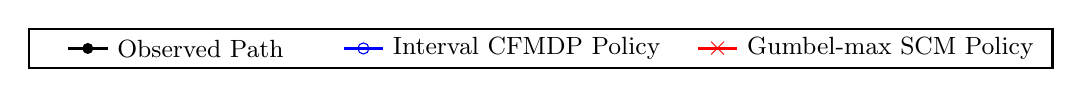
\begin{tikzpicture}[scale=1.0, every node/.style={scale=1.0}]
            \draw[thick, black] (-3, -0.25) rectangle (10, 0.25);
            %
            \draw[black, line width=1pt] (-2.5, 0.0) -- (-2,0.0);
            \fill[black] (-2.25,0.0) circle (2pt); %
            \node[right] at (-2,0.0) {\small Observed Path};
            
            %
            \draw[blue, line width=1pt] (1.0,0.0) -- (1.5,0.0);
            \node[draw=blue, circle, minimum size=4pt, inner sep=0pt] at (1.25,0.0) {}; %
            \node[right] at (1.5,0.0) {\small Interval CFMDP Policy};
            
            %
            \draw[red, line width=1pt] (5.5,0) -- (6,0);
            \node[red] at (5.75,0) {$\boldsymbol{\times}$}; %
            \node[right] at (6,0) {\small Gumbel-max SCM Policy};
        \end{tikzpicture}
    }\\
    %
    \subfigure[\footnotesize Lowest cumulative reward: Interval CFMDP ($312$), Gumbel-max SCM ($312$)]{%
        \resizebox{0.76\columnwidth}{!}{
             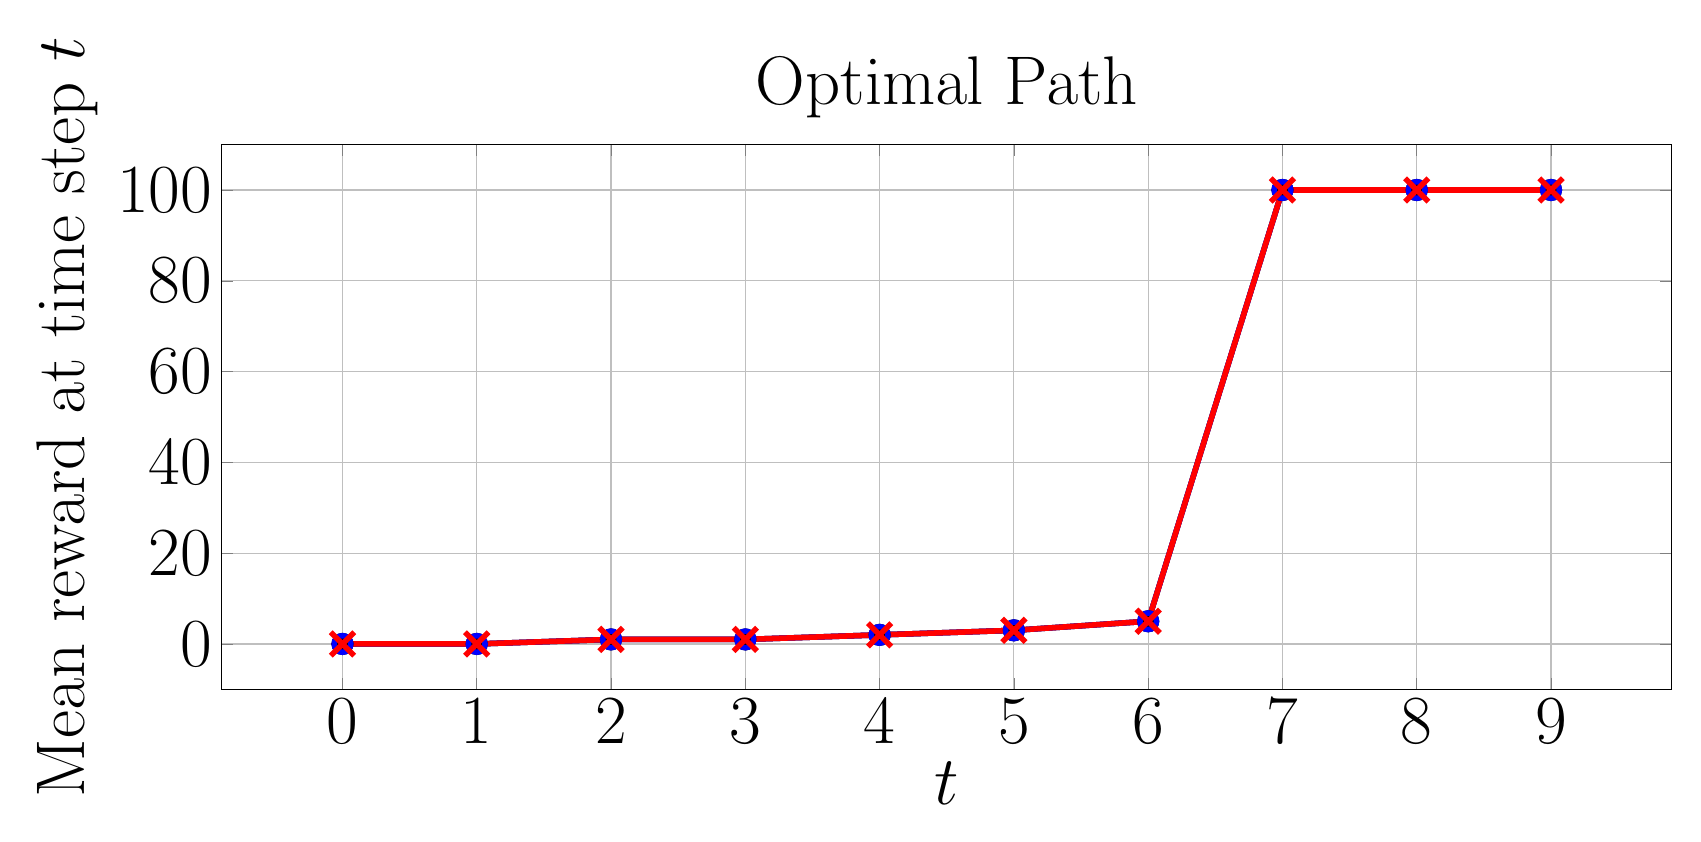
\begin{tikzpicture}
                \begin{axis}[
                    xlabel={$t$},
                    ylabel={Mean reward at time step $t$},
                    title={Optimal Path},
                    grid=both,
                    width=20cm, height=8.5cm,
                    every axis/.style={font=\Huge},
                    %
                ]
                \addplot[
                    color=black, %
                    mark=*, %
                    line width=2pt,
                    mark size=3pt,
                    error bars/.cd,
                    y dir=both, %
                    y explicit, %
                    error bar style={line width=1pt,solid},
                    error mark options={line width=1pt,mark size=4pt,rotate=90}
                ]
                coordinates {
                    (0, 0.0)  +- (0, 0.0)
                    (1, 0.0)  +- (0, 0.0) 
                    (2, 1.0)  +- (0, 0.0) 
                    (3, 1.0)  +- (0, 0.0)
                    (4, 2.0)  +- (0, 0.0)
                    (5, 3.0) +- (0, 0.0)
                    (6, 5.0) +- (0, 0.0)
                    (7, 100.0) +- (0, 0.0)
                    (8, 100.0) +- (0, 0.0)
                    (9, 100.0) +- (0, 0.0)
                };
                %
                \addplot[
                    color=blue, %
                    mark=o, %
                    line width=2pt,
                    mark size=3pt,
                    error bars/.cd,
                    y dir=both, %
                    y explicit, %
                    error bar style={line width=1pt,solid},
                    error mark options={line width=1pt,mark size=4pt,rotate=90}
                ]
                 coordinates {
                    (0, 0.0)  +- (0, 0.0)
                    (1, 0.0)  +- (0, 0.0) 
                    (2, 1.0)  +- (0, 0.0) 
                    (3, 1.0)  +- (0, 0.0)
                    (4, 2.0)  +- (0, 0.0)
                    (5, 3.0) +- (0, 0.0)
                    (6, 5.0) +- (0, 0.0)
                    (7, 100.0) +- (0, 0.0)
                    (8, 100.0) +- (0, 0.0)
                    (9, 100.0) +- (0, 0.0)
                };
                %
                \addplot[
                    color=red, %
                    mark=x, %
                    line width=2pt,
                    mark size=6pt,
                    error bars/.cd,
                    y dir=both, %
                    y explicit, %
                    error bar style={line width=1pt,solid},
                    error mark options={line width=1pt,mark size=4pt,rotate=90}
                ]
                coordinates {
                    (0, 0.0)  +- (0, 0.0)
                    (1, 0.0)  +- (0, 0.0) 
                    (2, 1.0)  +- (0, 0.0) 
                    (3, 1.0)  +- (0, 0.0)
                    (4, 2.0)  +- (0, 0.0)
                    (5, 3.0) +- (0, 0.0)
                    (6, 5.0) +- (0, 0.0)
                    (7, 100.0) +- (0, 0.0)
                    (8, 100.0) +- (0, 0.0)
                    (9, 100.0) +- (0, 0.0)
                };
                \end{axis}
            \end{tikzpicture}
         }
    }
    \hspace{1cm}
    \subfigure[\footnotesize Lowest cumulative reward: Interval CFMDP ($19$), Gumbel-max SCM ($-88$)]{%
         \resizebox{0.76\columnwidth}{!}{
            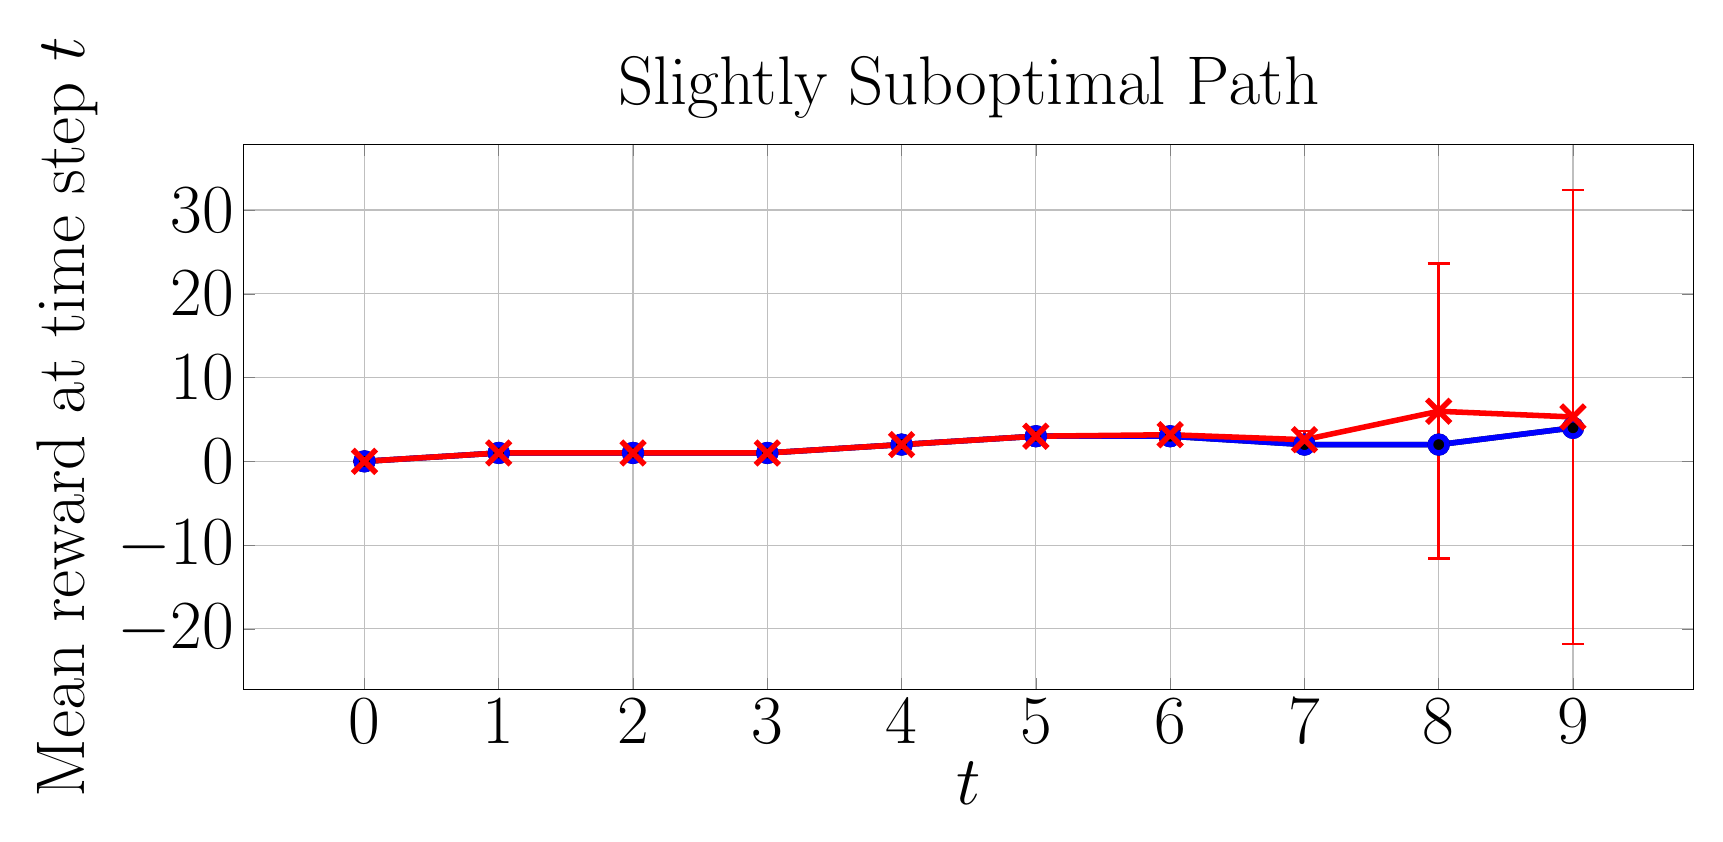
\begin{tikzpicture}
                \begin{axis}[
                    xlabel={$t$},
                    ylabel={Mean reward at time step $t$},
                    title={Slightly Suboptimal Path},
                    grid=both,
                    width=20cm, height=8.5cm,
                    every axis/.style={font=\Huge},
                    %
                ]
                \addplot[
                    color=black, %
                    mark=*, %
                    line width=2pt,
                    mark size=3pt,
                    error bars/.cd,
                    y dir=both, %
                    y explicit, %
                    error bar style={line width=1pt,solid},
                    error mark options={line width=1pt,mark size=4pt,rotate=90}
                ]
              coordinates {
                    (0, 0.0)  +- (0, 0.0)
                    (1, 1.0)  +- (0, 0.0) 
                    (2, 1.0)  +- (0, 0.0) 
                    (3, 1.0)  +- (0, 0.0)
                    (4, 2.0)  +- (0, 0.0)
                    (5, 3.0) +- (0, 0.0)
                    (6, 3.0) +- (0, 0.0)
                    (7, 2.0) +- (0, 0.0)
                    (8, 2.0) +- (0, 0.0)
                    (9, 4.0) +- (0, 0.0)
                };
                %
                \addplot[
                    color=blue, %
                    mark=o, %
                    line width=2pt,
                    mark size=3pt,
                    error bars/.cd,
                    y dir=both, %
                    y explicit, %
                    error bar style={line width=1pt,solid},
                    error mark options={line width=1pt,mark size=4pt,rotate=90}
                ]
              coordinates {
                    (0, 0.0)  +- (0, 0.0)
                    (1, 1.0)  +- (0, 0.0) 
                    (2, 1.0)  +- (0, 0.0) 
                    (3, 1.0)  +- (0, 0.0)
                    (4, 2.0)  +- (0, 0.0)
                    (5, 3.0) +- (0, 0.0)
                    (6, 3.0) +- (0, 0.0)
                    (7, 2.0) +- (0, 0.0)
                    (8, 2.0) +- (0, 0.0)
                    (9, 4.0) +- (0, 0.0)
                };
                %
                \addplot[
                    color=red, %
                    mark=x, %
                    line width=2pt,
                    mark size=6pt,
                    error bars/.cd,
                    y dir=both, %
                    y explicit, %
                    error bar style={line width=1pt,solid},
                    error mark options={line width=1pt,mark size=4pt,rotate=90}
                ]
                coordinates {
                    (0, 0.0)  +- (0, 0.0)
                    (1, 1.0)  +- (0, 0.0) 
                    (2, 1.0)  +- (0, 0.0) 
                    (3, 1.0)  +- (0, 0.0)
                    (4, 2.0)  += (0, 0.0)
                    (5, 3.0)  += (0, 0.0)
                    (6, 3.17847) += (0, 0.62606746) -= (0, 0.62606746)
                    (7, 2.5832885) += (0, 1.04598233) -= (0, 1.04598233)
                    (8, 5.978909) += (0, 17.60137623) -= (0, 17.60137623)
                    (9, 5.297059) += (0, 27.09227512) -= (0, 27.09227512)
                };
                \end{axis}
            \end{tikzpicture}
         }
    }\\[-1.5pt]
    \subfigure[\footnotesize Lowest cumulative reward: Interval CFMDP ($14$), Gumbel-max SCM ($-598$)]{%
         \resizebox{0.76\columnwidth}{!}{
             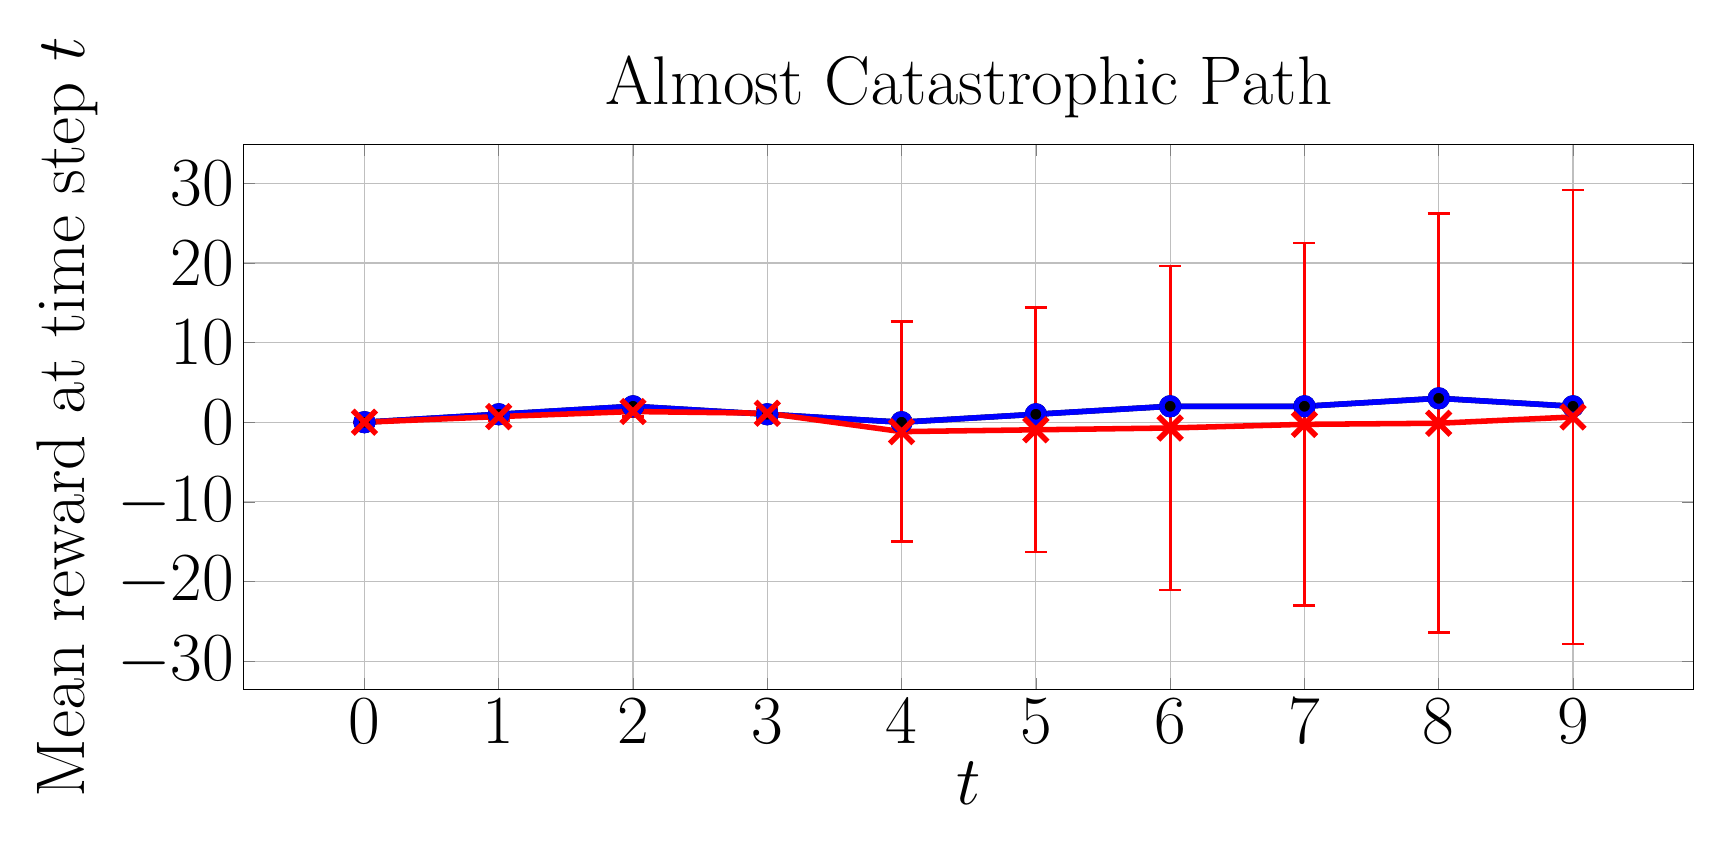
\begin{tikzpicture}
                \begin{axis}[
                    xlabel={$t$},
                    ylabel={Mean reward at time step $t$},
                    title={Almost Catastrophic Path},
                    grid=both,
                    width=20cm, height=8.5cm,
                    every axis/.style={font=\Huge},
                    %
                ]
                \addplot[
                    color=black, %
                    mark=*, %
                    line width=2pt,
                    mark size=3pt,
                    error bars/.cd,
                    y dir=both, %
                    y explicit, %
                    error bar style={line width=1pt,solid},
                    error mark options={line width=1pt,mark size=4pt,rotate=90}
                ]
                coordinates {
                    (0, 0.0)  +- (0, 0.0)
                    (1, 1.0)  +- (0, 0.0) 
                    (2, 2.0)  +- (0, 0.0) 
                    (3, 1.0)  +- (0, 0.0)
                    (4, 0.0)  +- (0, 0.0)
                    (5, 1.0) +- (0, 0.0)
                    (6, 2.0) +- (0, 0.0)
                    (7, 2.0) +- (0, 0.0)
                    (8, 3.0) +- (0, 0.0)
                    (9, 2.0) +- (0, 0.0)
                };
                %
                \addplot[
                    color=blue, %
                    mark=o, %
                    line width=2pt,
                    mark size=3pt,
                    error bars/.cd,
                    y dir=both, %
                    y explicit, %
                    error bar style={line width=1pt,solid},
                    error mark options={line width=1pt,mark size=4pt,rotate=90}
                ]
                coordinates {
                    (0, 0.0)  +- (0, 0.0)
                    (1, 1.0)  +- (0, 0.0) 
                    (2, 2.0)  +- (0, 0.0) 
                    (3, 1.0)  +- (0, 0.0)
                    (4, 0.0)  +- (0, 0.0)
                    (5, 1.0) +- (0, 0.0)
                    (6, 2.0) +- (0, 0.0)
                    (7, 2.0) +- (0, 0.0)
                    (8, 3.0) +- (0, 0.0)
                    (9, 2.0) +- (0, 0.0)
                };
                %
                \addplot[
                    color=red, %
                    mark=x, %
                    line width=2pt,
                    mark size=6pt,
                    error bars/.cd,
                    y dir=both, %
                    y explicit, %
                    error bar style={line width=1pt,solid},
                    error mark options={line width=1pt,mark size=4pt,rotate=90}
                ]
                coordinates {
                    (0, 0.0)  +- (0, 0.0)
                    (1, 0.7065655)  +- (0, 0.4553358) 
                    (2, 1.341673)  +- (0, 0.67091621) 
                    (3, 1.122926)  +- (0, 0.61281824)
                    (4, -1.1821935)  +- (0, 13.82444042)
                    (5, -0.952399)  +- (0, 15.35195457)
                    (6, -0.72672) +- (0, 20.33508414)
                    (7, -0.268983) +- (0, 22.77861454)
                    (8, -0.1310835) +- (0, 26.31013314)
                    (9, 0.65806) +- (0, 28.50670214)
                };
                %
            %
            %
            %
            %
            %
            %
            %
            %
            %
            %
            %
            %
            %
            %
            %
            %
            %
            %
                \end{axis}
            \end{tikzpicture}
         }
    }
    \hspace{1cm}
    \subfigure[\footnotesize Lowest cumulative reward: Interval CFMDP ($-698$), Gumbel-max SCM ($-698$)]{%
         \resizebox{0.76\columnwidth}{!}{
            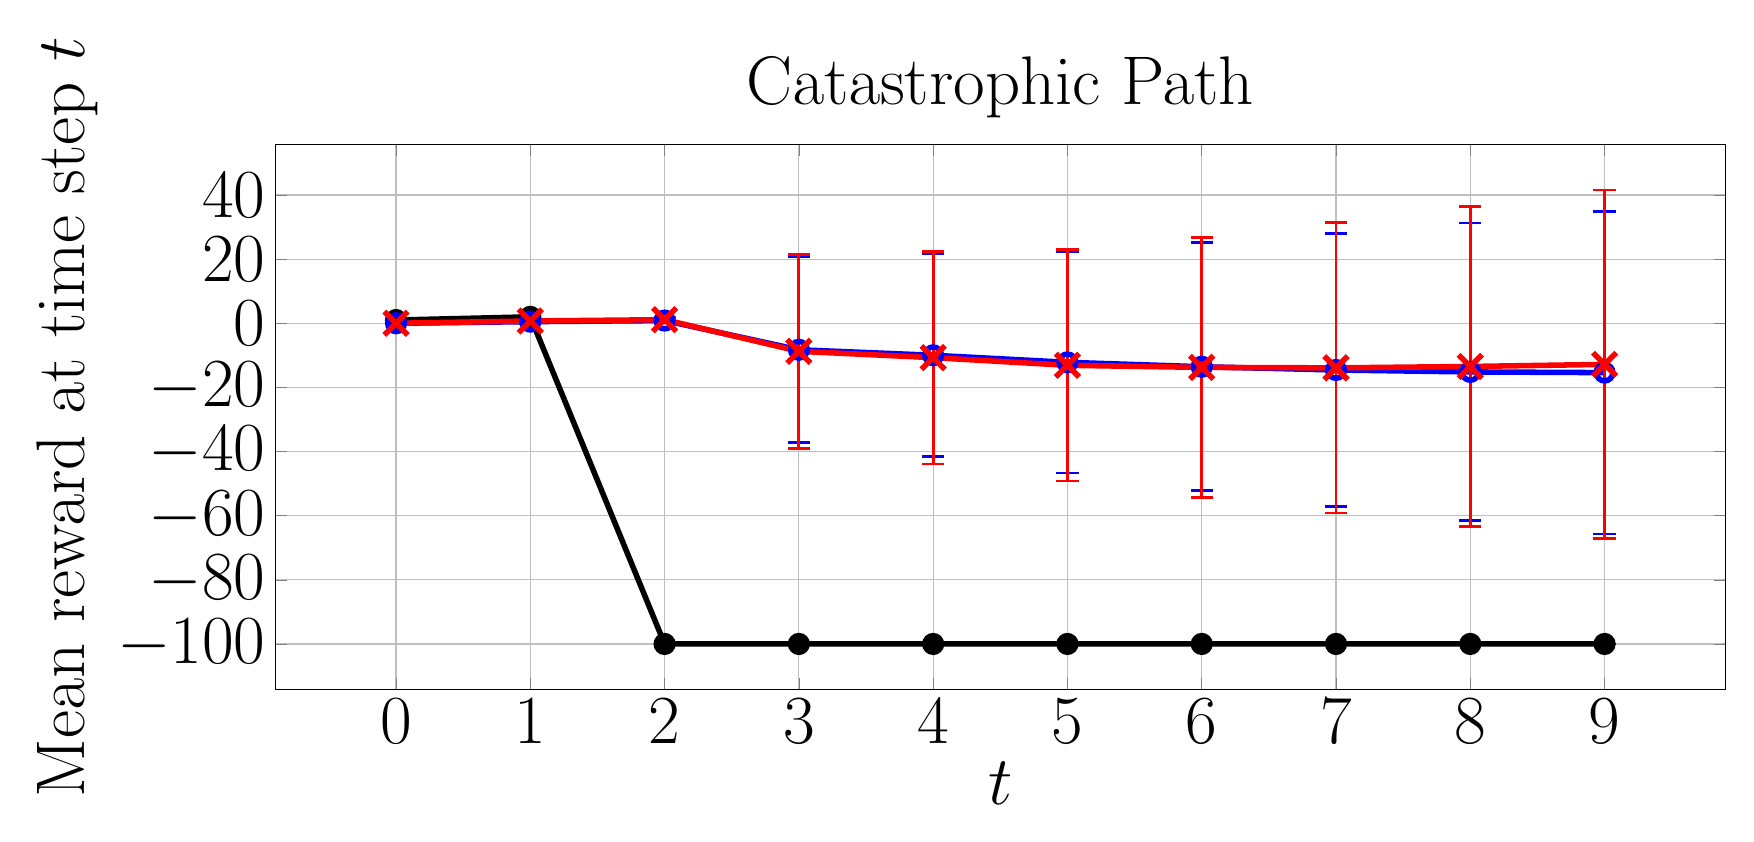
\begin{tikzpicture}
                \begin{axis}[
                    xlabel={$t$},
                    ylabel={Mean reward at time step $t$},
                    title={Catastrophic Path},
                    grid=both,
                    width=20cm, height=8.5cm,
                    every axis/.style={font=\Huge},
                    %
                ]
                \addplot[
                    color=black, %
                    mark=*, %
                    line width=2pt,
                    mark size=3pt,
                    error bars/.cd,
                    y dir=both, %
                    y explicit, %
                    error bar style={line width=1pt,solid},
                    error mark options={line width=1pt,mark size=4pt,rotate=90}
                ]
                coordinates {
                    (0, 1.0)  +- (0, 0.0)
                    (1, 2.0)  +- (0, 0.0) 
                    (2, -100.0)  +- (0, 0.0) 
                    (3, -100.0)  +- (0, 0.0)
                    (4, -100.0)  +- (0, 0.0)
                    (5, -100.0) +- (0, 0.0)
                    (6, -100.0) +- (0, 0.0)
                    (7, -100.0) +- (0, 0.0)
                    (8, -100.0) +- (0, 0.0)
                    (9, -100.0) +- (0, 0.0)
                };
                %
                \addplot[
                    color=blue, %
                    mark=o, %
                    line width=2pt,
                    mark size=3pt,
                    error bars/.cd,
                    y dir=both, %
                    y explicit, %
                    error bar style={line width=1pt,solid},
                    error mark options={line width=1pt,mark size=4pt,rotate=90}
                ]
                coordinates {
                    (0, 0.0)  +- (0, 0.0)
                    (1, 0.504814)  +- (0, 0.49997682) 
                    (2, 0.8439835)  +- (0, 0.76831917) 
                    (3, -8.2709165)  +- (0, 28.93656754)
                    (4, -9.981082)  +- (0, 31.66825363)
                    (5, -12.1776325) +- (0, 34.53463233)
                    (6, -13.556076) +- (0, 38.62845372)
                    (7, -14.574418) +- (0, 42.49603359)
                    (8, -15.1757075) +- (0, 46.41913968)
                    (9, -15.3900395) +- (0, 50.33563368)
                };
                %
                \addplot[
                    color=red, %
                    mark=x, %
                    line width=2pt,
                    mark size=6pt,
                    error bars/.cd,
                    y dir=both, %
                    y explicit, %
                    error bar style={line width=1pt,solid},
                    error mark options={line width=1pt,mark size=4pt,rotate=90}
                ]
                coordinates {
                    (0, 0.0)  +- (0, 0.0)
                    (1, 0.701873)  +- (0, 0.45743556) 
                    (2, 1.1227805)  +- (0, 0.73433129) 
                    (3, -8.7503255)  +- (0, 30.30257976)
                    (4, -10.722092)  +- (0, 33.17618589)
                    (5, -13.10721)  +- (0, 36.0648089)
                    (6, -13.7631645) +- (0, 40.56553451)
                    (7, -13.909043) +- (0, 45.23829402)
                    (8, -13.472517) +- (0, 49.96270296)
                    (9, -12.8278835) +- (0, 54.38618735)
                };
                %
            %
            %
            %
            %
            %
            %
            %
            %
            %
            %
            %
            %
            %
            %
            %
            %
            %
            %
                \end{axis}
            \end{tikzpicture}
         }
    }
    \caption{Average instant reward of CF paths induced by policies on GridWorld $p=0.4$.}
    \label{fig: reward p=0.4}
\end{figure*}

\subsection{Experimental Setup}
To compare policy performance, we measure the average rewards of counterfactual paths induced by our policy and the Gumbel-max policy by uniformly sampling $200$ counterfactual MDPs from the ICFMDP and generating $10,000$ counterfactual paths over each sampled CFMDP. \jl{Since the interval CFMDP depends on the observed path, we select $4$  paths of varying optimality to evaluate how the observed path impacts the performance of both policies: an optimal path, a slightly suboptimal path that could reach the optimal reward with a few changes, a catastrophic path that enters a catastrophic, terminal state with low reward, and an almost catastrophic path that was close to entering a catastrophic state.} When measuring the average probability bound widths and execution time needed to generate the ICFMDPs, we averaged over $20$ randomly generated observed paths
\footnote{Further training details are provided in Appendix \ref{app: training details}, and the code is provided at \href{https://github.com/ddv-lab/robust-cf-inference-in-MDPs}{https://github.com/ddv-lab/robust-cf-inference-in-MDPs}
%
%
.}.

\subsection{GridWorld}
\jl{The GridWorld MDP is a $4 \times 4$ grid where an agent must navigate from the top-left corner to the goal state in the bottom-right corner, avoiding a dangerous terminal state in the centre. At each time step, the agent can move up, down, left, or right, but there is a small probability (controlled by hyper-parameter $p$) of moving in an unintended direction. As the agent nears the goal, the reward for each state increases, culminating in a reward of $+100$ for reaching the goal. Entering the dangerous state results in a penalty of $-100$. We use two versions of GridWorld: a less stochastic version with $p=0.9$ (i.e., $90$\% chance of moving in the chosen direction) and a more stochastic version with $p=0.4$.}

\paragraph{GridWorld ($p=0.9$)}
When $p=0.9$, the counterfactual probability bounds are typically narrow (see Table \ref{tab:nonzero_probs} for average measurements). Consequently, as shown in Figure \ref{fig: reward p=0.9}, both policies are nearly identical and perform similarly well across the optimal, slightly suboptimal, and catastrophic paths.
%
However, for the almost catastrophic path, the interval CFMDP path is more conservative and follows the observed path more closely (as this is where the probability bounds are narrowest), which typically requires one additional step to reach the goal state than the Gumbel-max SCM policy.
%

\paragraph{GridWorld ($p=0.4$)}
\jl{When $p=0.4$, the GridWorld environment becomes more uncertain, increasing the risk of entering the dangerous state even if correct actions are chosen. Thus, as shown in Figure \ref{fig: reward p=0.4}, the interval CFMDP policy adopts a more conservative approach, avoiding deviation from the observed policy if it cannot guarantee higher counterfactual rewards (see the slightly suboptimal and almost catastrophic paths), whereas the Gumbel-max SCM is inconsistent: it can yield higher rewards, but also much lower rewards, reflected in the wide error bars.} For the catastrophic path, both policies must deviate from the observed path to achieve a higher reward and, in this case, perform similarly.
%
%
%
%
\subsection{Sepsis}
The Sepsis MDP \citep{oberst2019counterfactual} simulates trajectories of Sepsis patients. Each state consists of four vital signs (heart rate, blood pressure, oxygen concentration, and glucose levels), categorised as low, normal, or high.
and three treatments that can be toggled on/off at each time step (8 actions in total). Unlike \citet{oberst2019counterfactual}, we scale rewards based on the number of out-of-range vital signs, between $-1000$ (patient dies) and $1000$ (patient discharged). \jl{Like the GridWorld $p=0.4$ experiment, the Sepsis MDP is highly uncertain, as many states are equally likely to lead to optimal and poor outcomes. Thus, as shown in Figure \ref{fig: reward sepsis}, both policies follow the observed optimal and almost catastrophic paths to guarantee rewards are no worse than the observation.} However, improving the catastrophic path requires deviating from the observation. Here, the Gumbel-max SCM policy, on average, performs better than the interval CFMDP policy. But, since both policies have lower bounds clipped at $-1000$, neither policy reliably improves over the observation. In contrast, for the slightly suboptimal path, the interval CFMDP policy performs significantly better, shown by its higher lower bounds. 
Moreover, in these two cases, the worst-case counterfactual path generated by the interval CFMDP policy is better than that of the Gumbel-max SCM policy,
indicating its greater robustness.
%
\begin{figure*}
    \centering
     \resizebox{0.6\textwidth}{!}{
        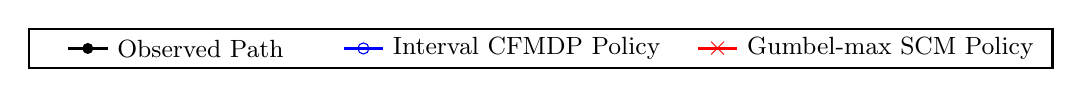
\begin{tikzpicture}[scale=1.0, every node/.style={scale=1.0}]
            \draw[thick, black] (-3, -0.25) rectangle (10, 0.25);
            %
            \draw[black, line width=1pt] (-2.5, 0.0) -- (-2,0.0);
            \fill[black] (-2.25,0.0) circle (2pt); %
            \node[right] at (-2,0.0) {\small Observed Path};
            
            %
            \draw[blue, line width=1pt] (1.0,0.0) -- (1.5,0.0);
            \node[draw=blue, circle, minimum size=4pt, inner sep=0pt] at (1.25,0.0) {}; %
            \node[right] at (1.5,0.0) {\small Interval CFMDP Policy};
            
            %
            \draw[red, line width=1pt] (5.5,0) -- (6,0);
            \node[red] at (5.75,0) {$\boldsymbol{\times}$}; %
            \node[right] at (6,0) {\small Gumbel-max SCM Policy};
        \end{tikzpicture}
    }\\
    \subfigure[\footnotesize Lowest cumulative reward: Interval CFMDP ($8000$), Gumbel-max SCM ($8000$)]{%
         \resizebox{0.76\columnwidth}{!}{
             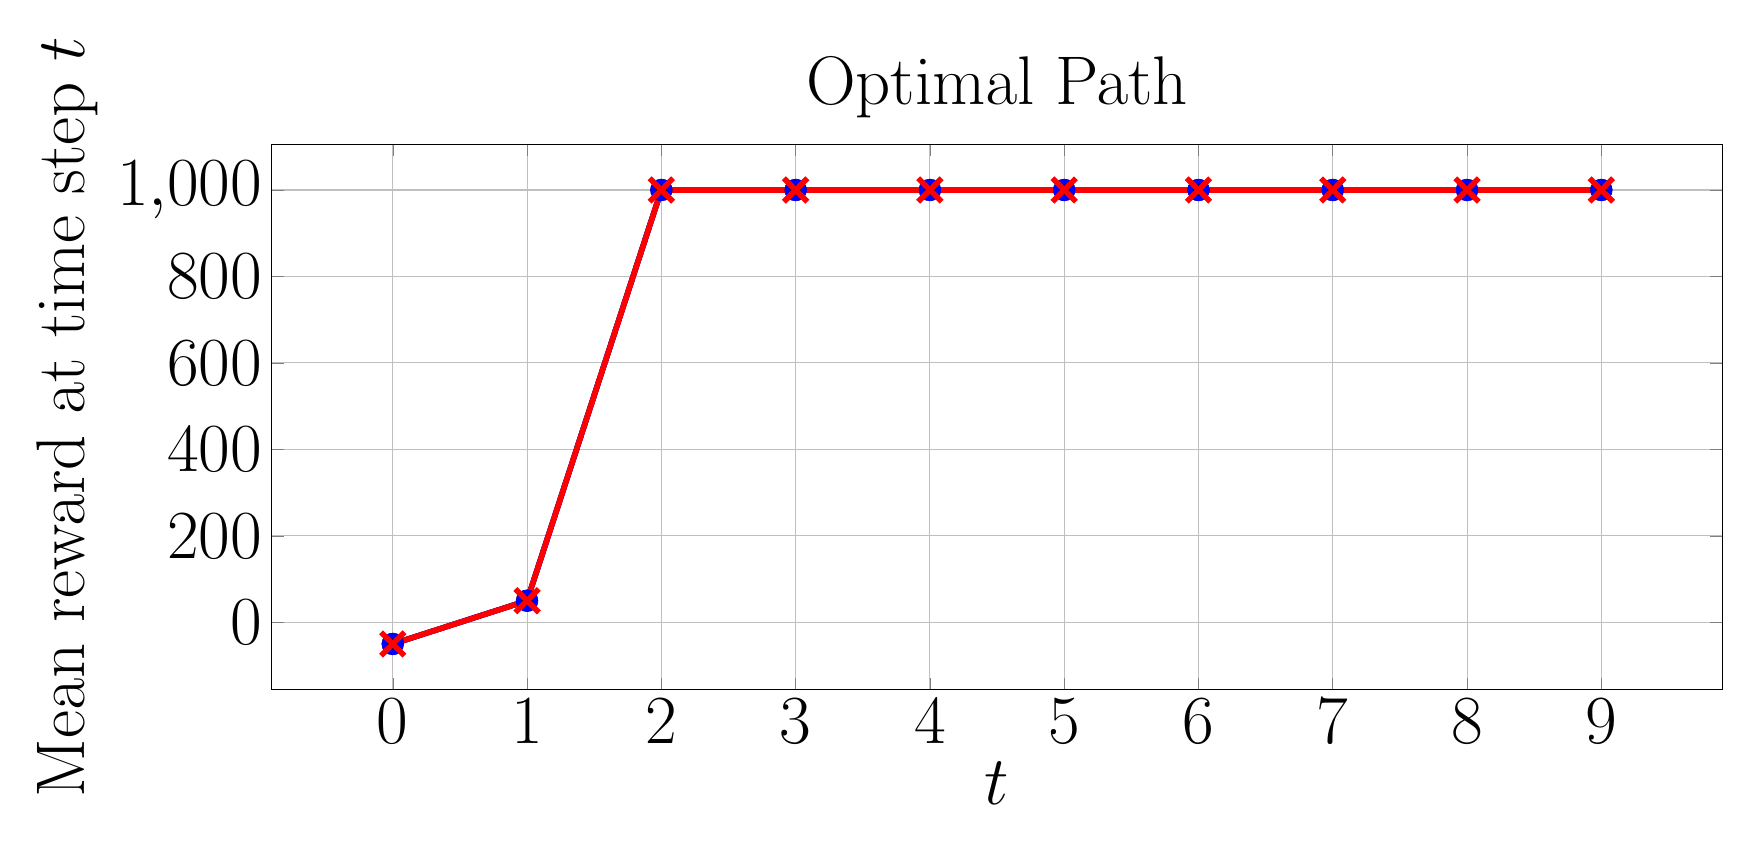
\begin{tikzpicture}
                \begin{axis}[
                    xlabel={$t$},
                    ylabel={Mean reward at time step $t$},
                    title={Optimal Path},
                    grid=both,
                    width=20cm, height=8.5cm,
                    every axis/.style={font=\Huge},
                    %
                ]
                \addplot[
                    color=black, %
                    mark=*, %
                    line width=2pt,
                    mark size=3pt,
                ]
                coordinates {
                    (0, -50.0)
                    (1, 50.0)
                    (2, 1000.0)
                    (3, 1000.0)
                    (4, 1000.0)
                    (5, 1000.0)
                    (6, 1000.0)
                    (7, 1000.0)
                    (8, 1000.0)
                    (9, 1000.0)
                };
                %
                \addplot[
                    color=blue, %
                    mark=o, %
                    line width=2pt,
                    mark size=3pt,
                    error bars/.cd,
                    y dir=both, %
                    y explicit, %
                    error bar style={line width=1pt,solid},
                    error mark options={line width=1pt,mark size=4pt,rotate=90}
                ]
                coordinates {
                    (0, -50.0)  +- (0, 0.0)
                    (1, 50.0)  +- (0, 0.0) 
                    (2, 1000.0)  +- (0, 0.0) 
                    (3, 1000.0)  +- (0, 0.0)
                    (4, 1000.0)  +- (0, 0.0)
                    (5, 1000.0) +- (0, 0.0)
                    (6, 1000.0) +- (0, 0.0)
                    (7, 1000.0) +- (0, 0.0)
                    (8, 1000.0) +- (0, 0.0)
                    (9, 1000.0) +- (0, 0.0)
                };
                %
                \addplot[
                    color=red, %
                    mark=x, %
                    line width=2pt,
                    mark size=6pt,
                    error bars/.cd,
                    y dir=both, %
                    y explicit, %
                    error bar style={line width=1pt,solid},
                    error mark options={line width=1pt,mark size=4pt,rotate=90}
                ]
                coordinates {
                    (0, -50.0)  +- (0, 0.0)
                    (1, 50.0)  +- (0, 0.0) 
                    (2, 1000.0)  +- (0, 0.0) 
                    (3, 1000.0)  +- (0, 0.0)
                    (4, 1000.0)  +- (0, 0.0)
                    (5, 1000.0) +- (0, 0.0)
                    (6, 1000.0) +- (0, 0.0)
                    (7, 1000.0) +- (0, 0.0)
                    (8, 1000.0) +- (0, 0.0)
                    (9, 1000.0) +- (0, 0.0)
                };
                %
                \end{axis}
            \end{tikzpicture}
         }
    }
    \hspace{1cm}
    \subfigure[\footnotesize Lowest cumulative reward: Interval CFMDP ($-5980$), Gumbel-max SCM ($-8000$)]{%
         \resizebox{0.76\columnwidth}{!}{
            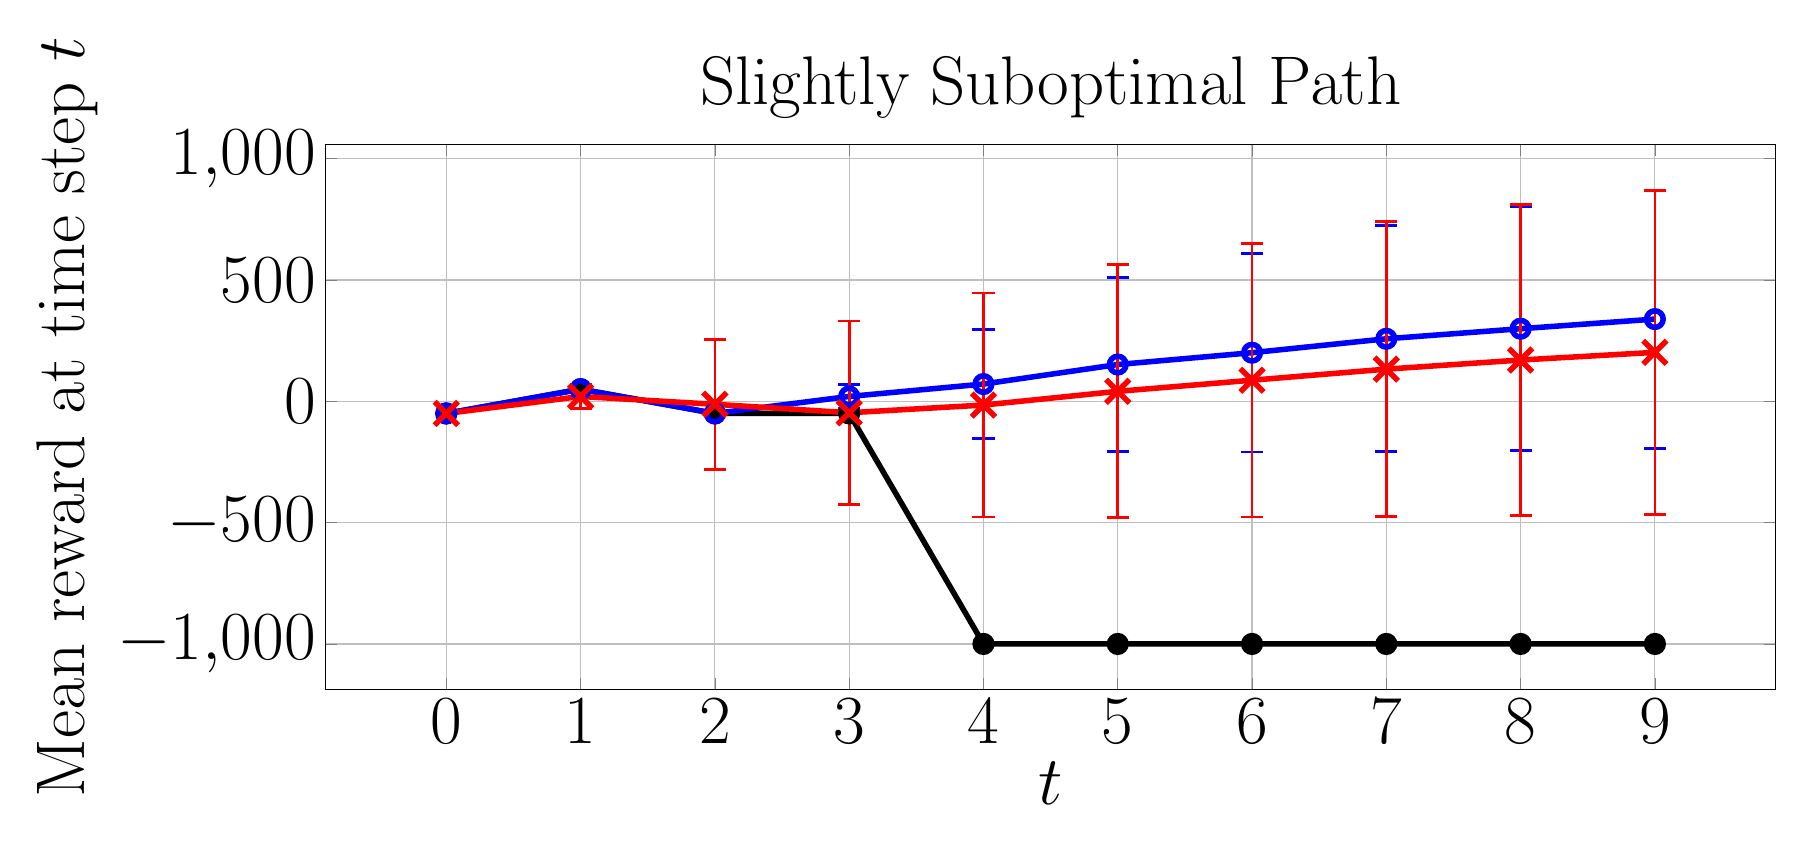
\begin{tikzpicture}
                \begin{axis}[
                    xlabel={$t$},
                    ylabel={Mean reward at time step $t$},
                    title={Slightly Suboptimal Path},
                    grid=both,
                    width=20cm, height=8.5cm,
                    every axis/.style={font=\Huge},
                    %
                ]
               \addplot[
                    color=black, %
                    mark=*, %
                    line width=2pt,
                    mark size=3pt,
                ]
                coordinates {
                    (0, -50.0)
                    (1, 50.0)
                    (2, -50.0)
                    (3, -50.0)
                    (4, -1000.0)
                    (5, -1000.0)
                    (6, -1000.0)
                    (7, -1000.0)
                    (8, -1000.0)
                    (9, -1000.0)
                };
                %
                \addplot[
                    color=blue, %
                    mark=o, %
                    line width=2pt,
                    mark size=3pt,
                    error bars/.cd,
                    y dir=both, %
                    y explicit, %
                    error bar style={line width=1pt,solid},
                    error mark options={line width=1pt,mark size=4pt,rotate=90}
                ]
                coordinates {
                    (0, -50.0)  +- (0, 0.0)
                    (1, 50.0)  +- (0, 0.0) 
                    (2, -50.0)  +- (0, 0.0) 
                    (3, 20.0631)  +- (0, 49.97539413)
                    (4, 71.206585)  +- (0, 226.02033693)
                    (5, 151.60797) +- (0, 359.23292559)
                    (6, 200.40593) +- (0, 408.86185176)
                    (7, 257.77948) +- (0, 466.10372804)
                    (8, 299.237465) +- (0, 501.82579506)
                    (9, 338.9129) +- (0, 532.06124996)
                };
                %
                \addplot[
                    color=red, %
                    mark=x, %
                    line width=2pt,
                    mark size=6pt,
                    error bars/.cd,
                    y dir=both, %
                    y explicit, %
                    error bar style={line width=1pt,solid},
                    error mark options={line width=1pt,mark size=4pt,rotate=90}
                ]
                coordinates {
                    (0, -50.0)  +- (0, 0.0)
                    (1, 20.00736)  +- (0, 49.99786741) 
                    (2, -12.282865)  +- (0, 267.598755) 
                    (3, -47.125995)  +- (0, 378.41755832)
                    (4, -15.381965)  +- (0, 461.77616558)
                    (5, 41.15459) +- (0, 521.53189262)
                    (6, 87.01595) +- (0, 564.22243126 )
                    (7, 132.62376) +- (0, 607.31338037)
                    (8, 170.168145) +- (0, 641.48013693)
                    (9, 201.813135) +- (0, 667.29441777)
                };
                %
                %
                %
                %
                %
                %
                %
                %
                %
                %
                %
                %
                %
                %
                %
                %
                %
                %
                %
                \end{axis}
            \end{tikzpicture}
         }
    }\\[-1.5pt]
    \subfigure[\footnotesize Lowest cumulative reward: Interval CFMDP ($100$), Gumbel-max SCM ($100$)]{%
         \resizebox{0.76\columnwidth}{!}{
             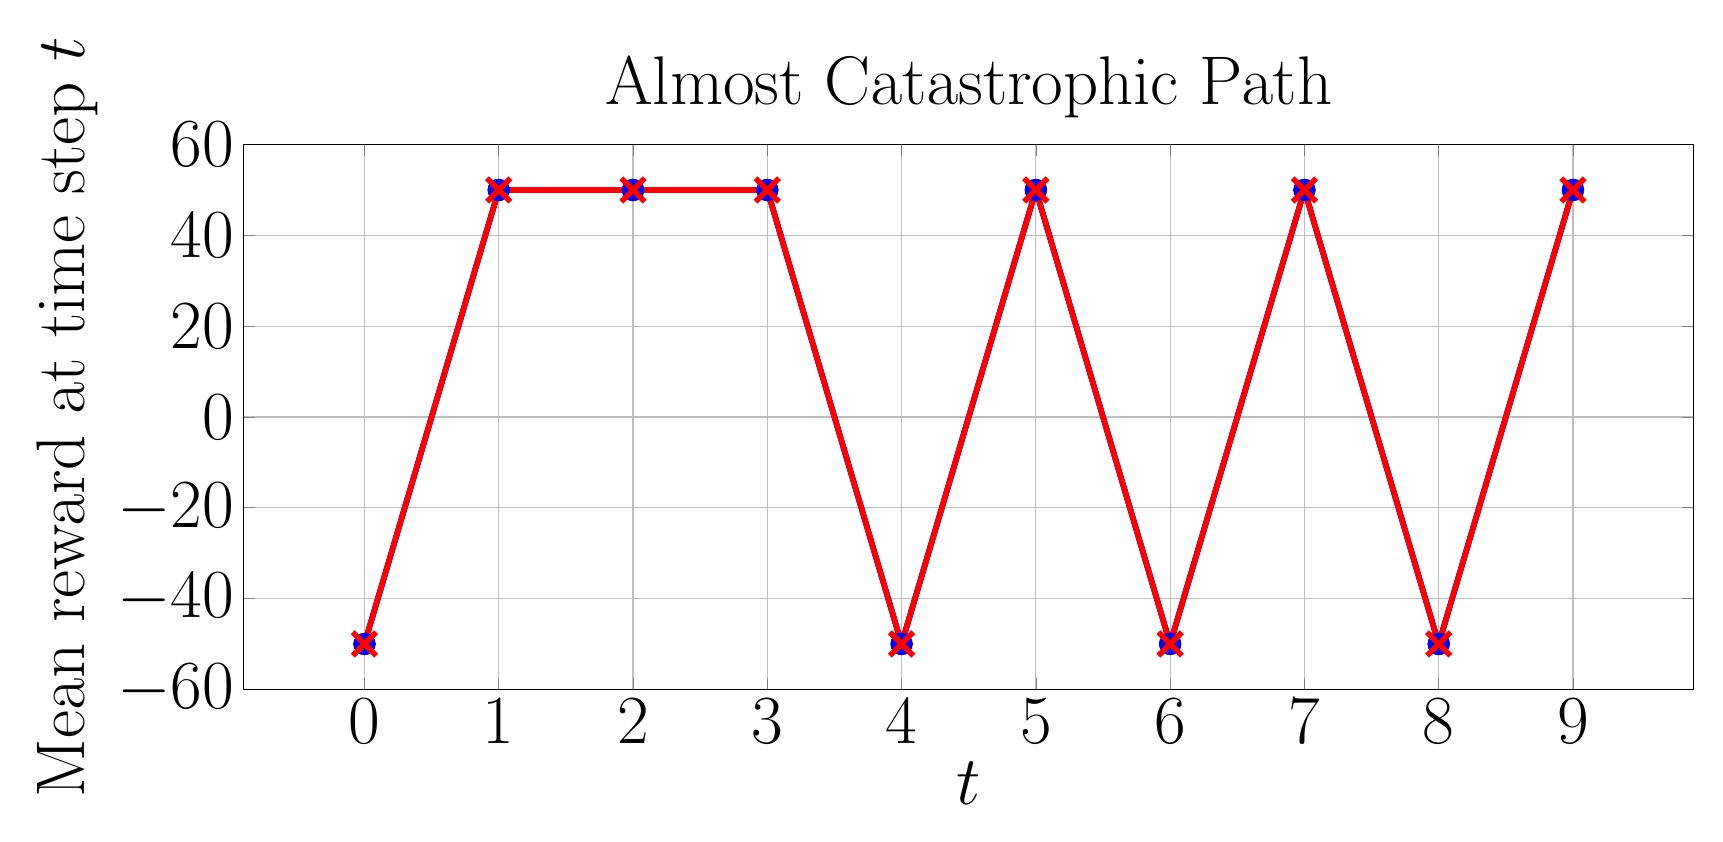
\begin{tikzpicture}
                \begin{axis}[
                    xlabel={$t$},
                    ylabel={Mean reward at time step $t$},
                    title={Almost Catastrophic Path},
                    grid=both,
                    every axis/.style={font=\Huge},
                    width=20cm, height=8.5cm,
                    %
                ]
               \addplot[
                    color=black, %
                    mark=*, %
                    line width=2pt,
                    mark size=3pt,
                ]
                coordinates {
                    (0, -50.0)
                    (1, 50.0)
                    (2, 50.0)
                    (3, 50.0)
                    (4, -50.0)
                    (5, 50.0)
                    (6, -50.0)
                    (7, 50.0)
                    (8, -50.0)
                    (9, 50.0)
                };
                %
                %
                \addplot[
                    color=blue, %
                    mark=o, %
                    line width=2pt,
                    mark size=3pt,
                    error bars/.cd,
                    y dir=both, %
                    y explicit, %
                    error bar style={line width=1pt,solid},
                    error mark options={line width=1pt,mark size=4pt,rotate=90}
                ]
                coordinates {
                    (0, -50.0)  +- (0, 0.0)
                    (1, 50.0)  +- (0, 0.0) 
                    (2, 50.0)  +- (0, 0.0) 
                    (3, 50.0)  +- (0, 0.0)
                    (4, -50.0)  +- (0, 0.0)
                    (5, 50.0) +- (0, 0.0)
                    (6, -50.0) +- (0, 0.0)
                    (7, 50.0) +- (0, 0.0)
                    (8, -50.0) +- (0, 0.0)
                    (9, 50.0) +- (0, 0.0)
                };
                %
                \addplot[
                    color=red, %
                    mark=x, %
                    line width=2pt,
                    mark size=6pt,
                    error bars/.cd,
                    y dir=both, %
                    y explicit, %
                    error bar style={line width=1pt,solid},
                    error mark options={line width=1pt,mark size=4pt,rotate=90}
                ]
                coordinates {
                    (0, -50.0)  +- (0, 0.0)
                    (1, 50.0)  +- (0, 0.0) 
                    (2, 50.0)  +- (0, 0.0) 
                    (3, 50.0)  +- (0, 0.0)
                    (4, -50.0)  +- (0, 0.0)
                    (5, 50.0) +- (0, 0.0)
                    (6, -50.0) +- (0, 0.0)
                    (7, 50.0) +- (0, 0.0)
                    (8, -50.0) +- (0, 0.0)
                    (9, 50.0) +- (0, 0.0)
                };
                %
                %
                %
                %
                %
                %
                %
                %
                %
                %
                %
                %
                %
                %
                %
                %
                %
                %
                %
                \end{axis}
            \end{tikzpicture}
         }
    }
    \hspace{1cm}
    \subfigure[\footnotesize Lowest cumulative reward: Interval CFMDP ($-7150$), Gumbel-max SCM ($-9050$)]{%
         \resizebox{0.76\columnwidth}{!}{
            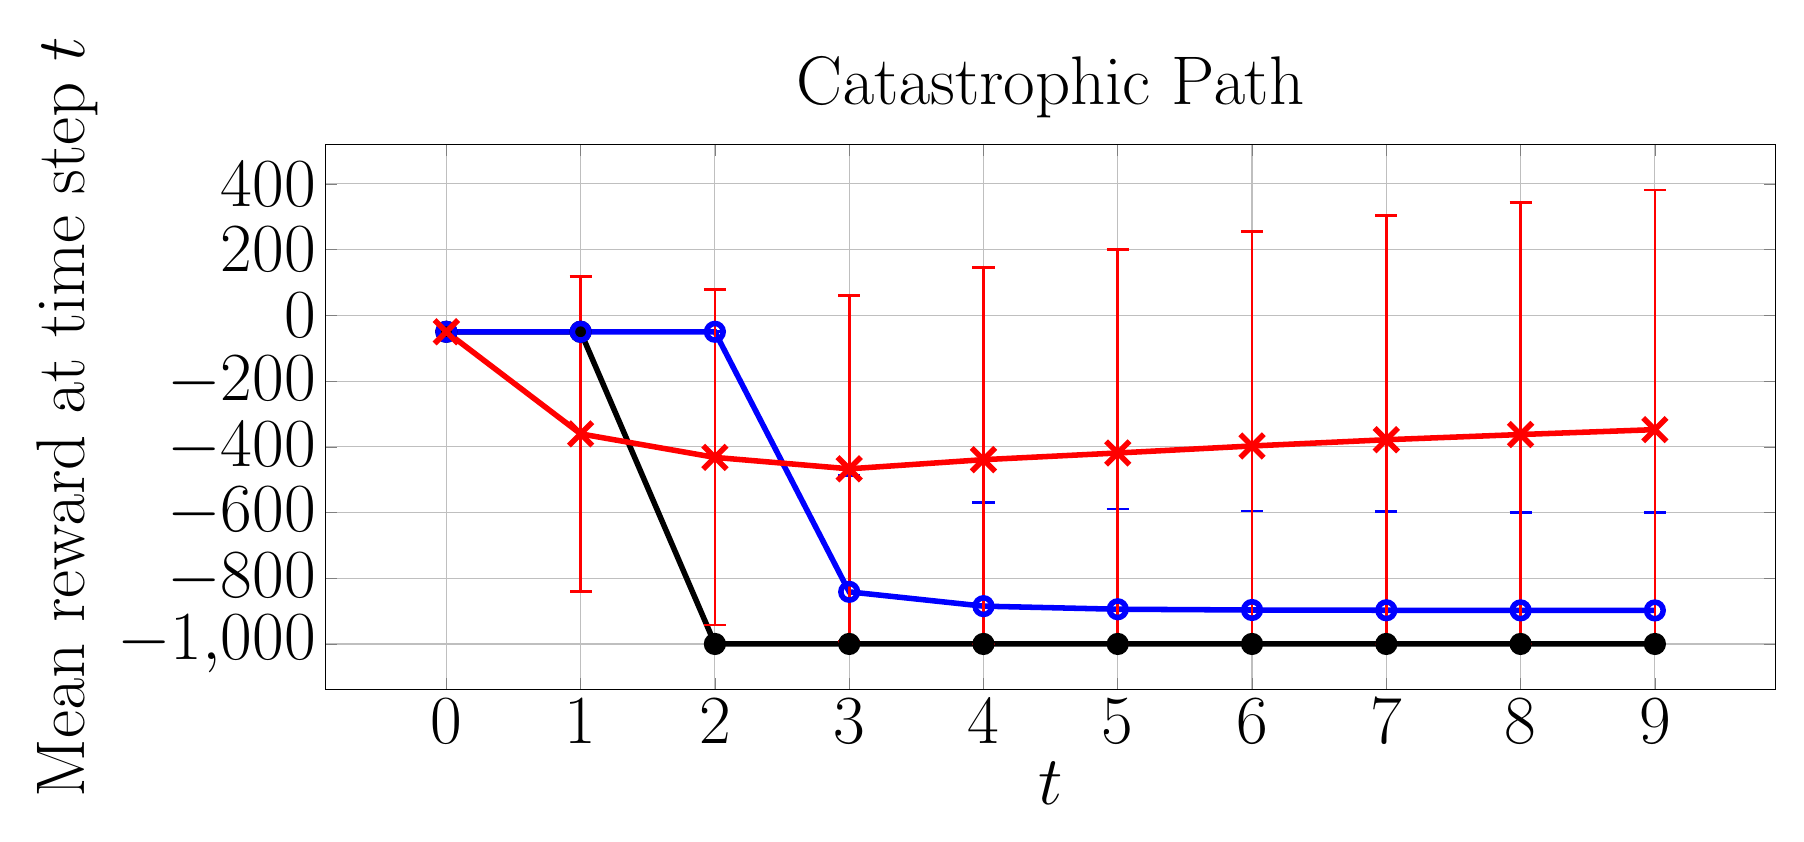
\begin{tikzpicture}
                \begin{axis}[
                    xlabel={$t$},
                    ylabel={Mean reward at time step $t$},
                    title={Catastrophic Path},
                    grid=both,
                    width=20cm, height=8.5cm,
                    every axis/.style={font=\Huge},
                    %
                ]
               \addplot[
                    color=black, %
                    mark=*, %
                    line width=2pt,
                    mark size=3pt,
                ]
                coordinates {
                    (0, -50.0)
                    (1, -50.0)
                    (2, -1000.0)
                    (3, -1000.0)
                    (4, -1000.0)
                    (5, -1000.0)
                    (6, -1000.0)
                    (7, -1000.0)
                    (8, -1000.0)
                    (9, -1000.0)
                };
                %
                %
                \addplot[
                    color=blue, %
                    mark=o, %
                    line width=2pt,
                    mark size=3pt,
                    error bars/.cd,
                    y dir=both, %
                    y explicit, %
                    error bar style={line width=1pt,solid},
                    error mark options={line width=1pt,mark size=4pt,rotate=90}
                ]
                coordinates {
                    (0, -50.0)  +- (0, 0.0)
                    (1, -50.0)  +- (0, 0.0) 
                    (2, -50.0)  +- (0, 0.0) 
                    (3, -841.440725)  += (0, 354.24605512) -= (0, 158.559275)
                    (4, -884.98225)  += (0, 315.37519669) -= (0, 115.01775)
                    (5, -894.330425) += (0, 304.88572805) -= (0, 105.669575)
                    (6, -896.696175) += (0, 301.19954514) -= (0, 103.303825)
                    (7, -897.4635) += (0, 299.61791279) -= (0, 102.5365)
                    (8, -897.77595) += (0, 298.80392585) -= (0, 102.22405)
                    (9, -897.942975) += (0, 298.32920557) -= (0, 102.057025)
                };
                %
                \addplot[
                    color=red, %
                    mark=x, %
                    line width=2pt,
                    mark size=6pt,
                    error bars/.cd,
                    y dir=both, %
                    y explicit, %
                    error bar style={line width=1pt,solid},
                    error mark options={line width=1pt,mark size=4pt,rotate=90}
                ]
            coordinates {
                    (0, -50.0)  +- (0, 0.0)
                    (1, -360.675265)  +- (0, 479.39812699) 
                    (2, -432.27629)  +- (0, 510.38620897) 
                    (3, -467.029545)  += (0, 526.36009628) -= (0, 526.36009628)
                    (4, -439.17429)  += (0, 583.96638919) -= (0, 560.82571)
                    (5, -418.82704) += (0, 618.43027478) -= (0, 581.17296)
                    (6, -397.464895) += (0, 652.67322574) -= (0, 602.535105)
                    (7, -378.49052) += (0, 682.85407033) -= (0, 621.50948)
                    (8, -362.654195) += (0, 707.01412023) -= (0, 637.345805)
                    (9, -347.737935) += (0, 729.29076479) -= (0, 652.262065)
                };
                %
                %
                %
                %
                %
                %
                %
                %
                %
                %
                %
                %
                %
                %
                %
                %
                %
                %
                %
                \end{axis}
            \end{tikzpicture}
         }
    }
    \caption{Average instant reward of CF paths induced by policies on Sepsis.}
    \label{fig: reward sepsis}
\end{figure*}

%
%
%
\subsection{Interval CFMDP Bounds}
%
%
Table \ref{tab:nonzero_probs} presents the mean counterfactual probability bound widths (excluding transitions where the upper bound is $0$) for each MDP, averaged over 20 observed paths. We compare the bounds under counterfactual stability (CS) and monotonicity (M) assumptions, CS alone, and no assumptions. This shows that the assumptions marginally reduce the bound widths, indicating the assumptions tighten the bounds without excluding too many causal models, as intended.
\renewcommand{\arraystretch}{1}

\begin{table}
\centering
\caption{Mean width of counterfactual probability bounds}
\resizebox{0.8\columnwidth}{!}{%
\begin{tabular}{|c|c|c|c|}
\hline
\multirow{2}{*}{\textbf{Environment}} & \multicolumn{3}{c|}{\textbf{Assumptions}} \\ \cline{2-4}
 & \textbf{CS + M} & \textbf{CS} & \textbf{None\tablefootnote{\jl{Equivalent to \citet{li2024probabilities}'s bounds (see Section \ref{sec: equivalence with Li}).}}} \\ \hline
\textbf{GridWorld} ($p=0.9$) & 0.0817 & 0.0977 & 0.100 \\ \hline
\textbf{GridWorld} ($p=0.4$) & 0.552  & 0.638  & 0.646 \\ \hline
\textbf{Sepsis} & 0.138 & 0.140 & 0.140 \\ \hline
\end{tabular}
}
\label{tab:nonzero_probs}
\end{table}


\subsection{Execution Times}
Table \ref{tab: times} compares the average time needed to generate the interval CFMDP vs.\ the Gumbel-max SCM CFMDP for 20 observations.
The GridWorld algorithms were run single-threaded, while the Sepsis experiments were run in parallel.
Generating the interval CFMDP is significantly faster as it uses exact analytical bounds, whereas the Gumbel-max CFMDP requires sampling from the Gumbel distribution to estimate counterfactual transition probabilities. \jl{Since constructing the counterfactual MDP models is the main bottleneck in both approaches, ours is more efficient overall and suitable for larger MDPs.}
\begin{table}
\centering
\caption{Mean execution time to generate CFMDPs}
\resizebox{0.99\columnwidth}{!}{%
\begin{tabular}{|c|c|c|}
\hline
\multirow{2}{*}{\textbf{Environment}} & \multicolumn{2}{c|}{\textbf{Mean Execution Time (s)}} \\ \cline{2-3} 
                                      & \textbf{Interval CFMDP} & \textbf{Gumbel-max CFMDP} \\ \hline
\textbf{GridWorld ($p=0.9$) }                  & 0.261                   & 56.1                      \\ \hline
\textbf{GridWorld ($p=0.4$)  }                 & 0.336                   & 54.5                      \\ \hline
\textbf{Sepsis}                                 & 688                     & 2940                      \\ \hline
\end{tabular}%
}
\label{tab: times}
\end{table}




\section{Conclusion}

We systematically evaluated the role of consensus and voting decision protocols across three knowledge and three reasoning tasks.
Our study assessed how the number of discussion rounds and agents influences task performance.
We propose two new methods to improve answer diversity during multi-agent discussions and decisions, i.e., \acf{AAD} and \acf{CI}. 
\ac{AAD} requires each agent to contribute draft ideas at the beginning of the discussion, and \ac{CI} encourages independent reasoning steps by limiting communication between agents and only allowing them to exchange possible solutions after each turn.

Our findings show that voting performs well on reasoning tasks, outperforming consensus by up to $13.2\%$, and outperforming a single \ac{CoT} baseline by 10.4\%.
This is likely because voting-based protocols allow agents to explore multiple reasoning paths instead of a single one, as in consensus.
In comparison, consensus outperforms voting in knowledge tasks by up to $2.8\%$, because it improves fact-checking by requiring at least the agreement of the majority of agents.
Increasing the number of agents in the discussion improved task performance, while increasing the number of discussion rounds before voting decreased performance.
\ac{AAD} improved performance by up to $3.3\%$, and \ac{CI} by up to $7.4\%$ over default multi-agent debate baseline, and 6.1\% and 10.2\% over single model \ac{CoT} baseline respectively.
Our new methods enhance answer diversity and reveal a connection between answer diversity and task performance.

Future work could explore other characteristics influencing decisions, such as power relations between managers and employees. 
This could also involve examining personas within this hierarchical structure to investigate whether dominant or affectionate leaders are more effective in leading discussions \citep{AMES2009111}.


We recommend using voting in reasoning tasks and consensus in knowledge tasks, scaling up the number of agents instead of the number of rounds, and increasing the diversity of answers between agents using \ac{AAD} and \ac{CI}.

\section*{Limitations} %
Multi-agent debates are computationally expensive because they require a message from each agent in each round, quickly leading to hundreds of forward passes per model.
Because of the high computational cost and the range of decision protocols and tasks in our work, we used sampled subsets of the datasets, which can lead to some variance.
To control for that variance, we sampled with a 95\% confidence level and calculated the standard deviation of three independent runs.%
Overall, the results were markedly higher than what could be explained by the standard deviation.
More details about the dataset and other parameters can be found in \Cref{appendix:datasets}.
Despite efforts to improve answer diversity, agents often converged on similar responses, suggesting that more advanced techniques to encourage independent solutions are needed in the future.


% \section{Acknowledgment}
\begin{acks}
This material was supported by the U.S. Dept. of Energy, Office
of Science, Advanced Scientific Computing Research (ASCR), under contracts DE-AC02-06CH11357 and DE-SC002\newline 4207.
\end{acks}
\bibliographystyle{ACM-Reference-Format}
\bibliography{acmart}
\end{document}
\endinput
%%
%% End of file `sample-sigplan.tex'.
